\chapter{KIẾN THỨC NỀN TẢNG VÀ KHẢO SÁT}
\ifpdf
    \graphicspath{{Chapter2/Chapter2Figs/PNG/}{Chapter2/Chapter2Figs/PDF/}{Chapter2/Chapter2Figs/}}
\else
    \graphicspath{{Chapter2/Chapter2Figs/EPS/}{Chapter2/Chapter2Figs/}}
\fi

Để có thể thực hiện được những mục tiêu cụ thể đã đề ra trong chương đầu tiên, chương này đồ án sẽ trình bày về các kiến thức nền tảng cho việc xây dựng đề tài, đồng thời cũng thực hiện khảo sát các hệ thống, phần mềm có liên quan.

Đầu tiên đồ án sẽ nói về các kiến thức cơ bản về mạng WiFi như định nghĩa, các mô hình mạng, các loại khung và các tiêu chuẩn mã hóa. Tiếp theo là các tấn công điển hình trong mạng WiFi, chúng có đặc điểm gì và vì sao có thể phát hiện được các tấn công đó đang diễn ra. Kế tiếp là tổng quan về hệ thống phát hiện xâm nhập, từ đó tìm hiểu sự khác nhau giữa hệ thống phát hiện xâm nhập thông thường và hệ thống phát hiện xâm nhập cho mạng WiFi (hay mạng không dây). Cuối chương đồ án sẽ khảo sát về các hệ thống phát hiện xâm nhập đã được phát triển và các kiến thức liên quan để phục vụ cho việc thiết kế hệ thống WIDS đề xuất ở chương sau.

\section{Tổng quan về mạng WiFi}

\subsection{Giới thiệu}
\emph{WiFi} là tên rút gọn của Wireless Fidelity, dùng để chỉ các loại mạng thuộc chuẩn mạng không dây IEEE 802.11. WiFi cũng là chuẩn công nghiệp cho các sản phẩm được định nghĩa bởi WiFi Alliance và phù hợp với chuẩn IEEE 802.11~\cite{varma2006wireless}.

Chuẩn IEEE 802.11 do Viện Kỹ thuật Điện và Điện tử (IEEE) phát triển, bao gồm các đặc tả kỹ thuật liên quan đến hệ thống mạng không dây. Chuẩn IEEE 802.11 mô tả một liên lạc "truyền qua không khí" sử dụng sóng vô tuyến để truyền nhận tín hiệu giữa một thiết bị không dây và tổng đài hoặc điểm truy cập, hoặc giữa hai hay nhiều thiết bị không dây với nhau~\cite{ieee2012802}. Vì vậy, đồ án này sẽ dùng các thuật ngữ \emph{mạng không dây}, \emph{mạng 802.11}, \emph{mạng WiFi} với ý nghĩa như nhau, dùng để chỉ mạng WiFi.

Các đặc tả của IEEE 802 tập trung vào hai lớp thấp nhất trong mô hình OSI là lớp liên kết dữ liệu (Datalink) và lớp vật lý (Physical). Hình~\ref{fig:80211-reference-osi} thể hiện kiến trúc của chuẩn 802.11 và sự tham chiếu trong mô hình OSI.

\begin{figure}[!htbp]
    \centering
    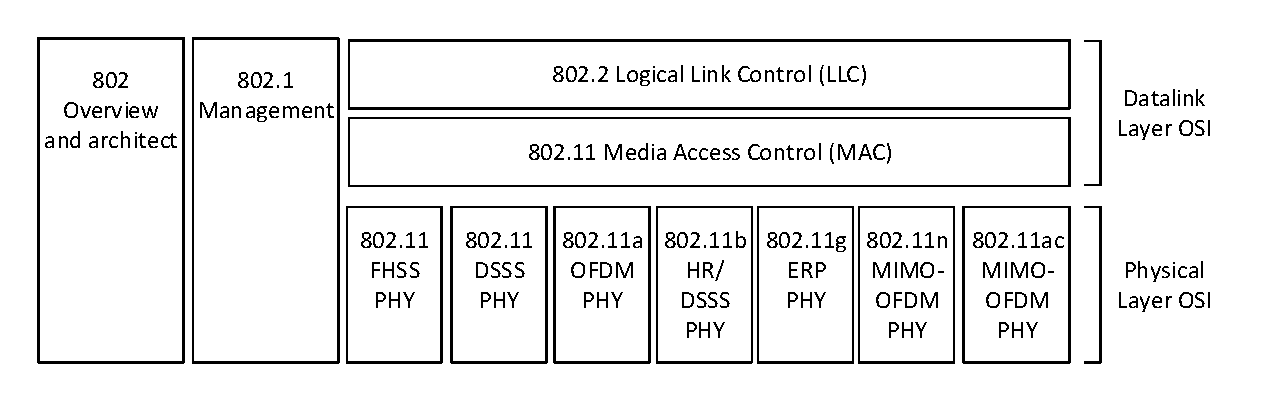
\includegraphics[width=1.0\textwidth]{80211-reference-osi}
    \caption{
        \label{fig:80211-reference-osi}
        Kiến trúc 802.11 và sự tham chiếu trong mô hình OSI}% ~\cite{gast2005802}
\end{figure}

Hình~\ref{fig:80211-reference-osi} cho thấy chuẩn 802.2 đặc tả lớp con điều khiển liên kết luận lý (LLC) chung, được sử dụng bởi các lớp bên dưới thuộc mọi công nghệ LAN, nhằm tạo tính tương thích giữa chúng cũng như cung cấp cái nhìn trong suốt từ các lớp bên trên (từ lớp ứng dụng cho tới lớp mạng). Bên cạnh đó, các mạng 802 đều có một lớp con điều khiển truy cập thiết bị (MAC) và lớp vật lý (PHY) riêng, trong đó:
\begin{itemize}
\item Lớp con điều khiển truy cập thiết bị (MAC) là một tập các luật xác định cách thức truy cập thiết bị phần cứng và gửi dữ liệu.
\item Lớp vật lý (PHY) đảm nhiệm chi tiết việc gửi và nhận dữ liệu bằng thiết bị phần cứng.
\end{itemize}

Các chuẩn thường gặp như 802.11a, 802.11b, 802.11g, 802.11n và gần đây là 802.11ac được dùng để đặc tả những yêu cầu kỹ thuật khác nhau ở lớp vật lý.

\subsection{Các mô hình mạng}

\subsubsection{Các thành phần chính}
Mạng WiFi gồm bốn thành phần vật lý chính, được tóm tắt như Hình~\ref{fig:80211-architecture}.

\begin{itemize}
\item \emph{Trạm (Station - STA):} các trạm tham gia truyền dữ liệu trong mạng thông qua card mạng không dây như máy tính xách tay, điện thoại thông minh.
\item \emph{Điểm truy cập (Access Point - AP):} là thiết bị trung gian, điều khiển kết nối không dây trong mạng WiFi cũng như giữa chúng với mạng có dây.

\begin{figure}[H]
    \centering
    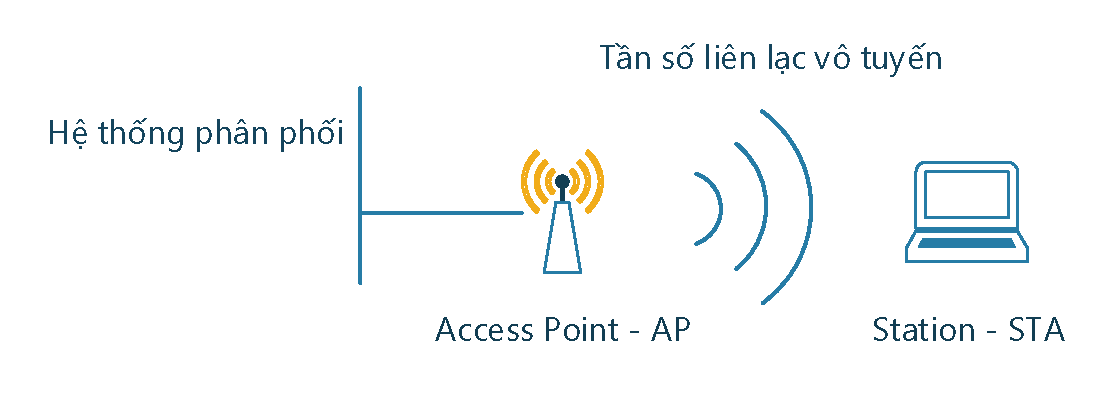
\includegraphics[width=1.0\textwidth]{80211-architecture}
    \caption{
        \label{fig:80211-architecture}
        Các thành phần vật lý của mạng WiFi}% ~\cite{gast2005802}
\end{figure}

\item \emph{Tần số liên lạc vô tuyến (Wireless Medium):} tùy theo đặc tả kỹ thuật của chuẩn cụ thể, cũng như loại sóng vô tuyến được sử dụng, các thiết bị sẽ cần một tần số liên lạc vô tuyến nhất định để truyền dữ liệu trong mạng WiFi.
\item \emph{Hệ thống phân phối (Distribution System):} bằng cách nối thêm các điểm truy cập, mạng WiFi có thể bao phủ một phạm vi lớn hơn.
\end{itemize}

\subsubsection{Các mô hình mạng}
Trong mạng WiFi có hai mô hình mạng phổ biến: mô hình mạng độc lập (Ad-hoc hay Independent BSS) và mô hình mạng cơ cở (Infrastructure BSS). Trong mô hình mạng độc lập, các STA tập trung lại trong một không gian nhỏ để hình thành nên kết nối ngang hàng giữa chúng.%~\cite{gast2005802}.

Các STA trong mô hình mạng cơ cở liên lạc với nhau thông qua AP. AP là điểm trung tâm quản lý mọi sự giao tiếp trong mạng. Để giao tiếp với nhau, các STA khác phải gửi các khung đến AP, sau đó AP sẽ gửi đến STA nhận. Một mô hình mạng cơ sở đơn giản với một AP được gọi là tập dịch vụ cơ bản (Basic Service Set - BSS). Một mạng có nhiều hơn một AP tạo thành một mạng gọi là tập dịch vụ mở rộng (Extended Service Set - ESS).%~\cite{gast2005802}.

Trong mô hình mạng cơ sở có hai khái niệm cơ bản là định danh tập dịch vụ (Service Set Identifier - SSID) và định danh tập dịch vụ cơ bản (Basic Service Set Identifier - BSSID). SSID là một định danh duy nhất gồm 32 ký tự chứa trong tiêu đề hoặc gói tin được gửi trên mạng hoạt động như một mật khẩu khi STA cố gắng thiết lập kết nối với BSS~\cite{vasseur2010interconnecting}. SSID phân biệt một mạng WiFi này với một mạng WiFi khác, vì vậy tất cả các AP và thiết bị cố gắng kết nối với một mạng WiFi cụ thể phải sử dụng cùng một SSID. SSID cũng được coi là tên mạng vì nó có thể dễ dàng đọc được. BSSID là một trường có độ dài 48 bit giống như địa chỉ MAC, trường này là định danh duy nhất cho mỗi BSS, giá trị của nó chính là địa chỉ MAC của AP~\cite{ieee2007802}.

\subsection{Khung quản lý}
\newcommand\tab[1][2.5mm]{\hspace*{#1}}
Chuẩn 802.11 định nghĩa một số loại khung (frame) khác nhau để các STA và AP sử dụng để liên lạc, cũng như quản lý và kiểm soát các liên kết không dây. Có ba loại khung chính, trong đó khung quản lý (management frame) cho phép các STA thiết lập và duy trì liên lạc. Dưới đây là một số loại phụ của khung quản lý~\cite{geier2001wireless}:
\begin{itemize}
\item \emph{Khung yêu cầu liên kết (association request):} \tab Một STA sẽ gửi khung này đến một AP nếu muốn liên kết với AP đó. Một STA sẽ được liên kết với một AP sau khi AP đó cho phép.

\item \emph{Khung đáp ứng liên kết (association response):} \tab Sau khi một AP nhận được một khung yêu cầu liên kết, AP sẽ gửi một khung đáp ứng liên kết để cho biết có chấp nhận sự liên kết với STA gửi hay không.

\item \emph{Khung yêu cầu liên kết lại (reassociation request):} \tab Một STA sẽ gửi khung này đến một AP nếu nó muốn liên kết lại với AP đó. Sự liên kết lại có thể xảy ra nếu một STA di chuyển ra ngoài phạm vi của một AP và trong phạm vi của một AP khác. STA sẽ cần liên kết với AP mới để AP mới biết rằng nó sẽ cần thương lượng chuyển tiếp các khung dữ liệu từ AP cũ.

\item \emph{Khung đáp ứng liên kết lại (reassociation response):} \tab Sau khi một AP nhận được một khung yêu cầu liên kết lại, AP sẽ gửi một khung đáp ứng liên kết lại để cho biết có chấp nhận việc liên kết lại với STA gửi không.

\item \emph{Khung yêu cầu thăm dò (probe request):} \tab Một STA gửi một khung yêu cầu thăm dò để thu thập thông tin từ một STA hoặc AP khác. Ví dụ, một STA có thể gửi một khung yêu cầu thăm dò để xác định có một AP nào đó hiện diện hay không.

\item \emph{Khung đáp ứng thăm dò (probe response):} \tab Nếu STA hoặc AP nhận được một khung yêu cầu thăm dò, nó sẽ trả lời STA gửi bằng một khung đáp ứng thăm dò có chứa các thông số cụ thể về chính nó (chẳng hạn như các tham số cho trải phổ nhảy tần và trải phổ trực tiếp ở lớp vật lý).

\item \emph{Khung báo hiệu (beacon):} \tab Trong mô hình mạng cơ sở, một AP định kỳ gửi một báo hiệu (theo tham số aBeaconPeriod trong MIB) cung cấp sự đồng bộ giữa các STA sử dụng lớp PHY giống nhau. Beacon bao gồm một dấu thời gian mà tất cả các STA sử dụng để cập nhật những gì 802.11 định nghĩa như một bộ đếm thời gian đồng bộ hóa chức năng (TSF). Nếu một AP hỗ trợ chức năng điều phối điểm, thì nó sử dụng một khung báo hiệu để thông báo sự bắt đầu của thời kỳ không tranh chấp. Nếu mạng có mô hình mạng độc lập (tức là nó không có AP), tất cả các STA định kỳ gửi báo hiệu cho mục đích đồng bộ hóa.

\item \emph{Khung thông báo chỉ dẫn lưu thông (Announcement Traffic Indication Message - ATIM):} \tab Một STA với khả năng lưu tạm các khung cho các STA khác, sẽ gửi một khung ATIM cho mỗi STA thông qua cửa sổ ATIM, ngay sau khi một thăm dò được truyền. Sau đó, STA truyền những khung này tới những STA nhận thích hợp. Việc truyền tải các khung ATIM cảnh báo cho các STA đang trong trạng thái ngủ, để chuyển sang trạng thái thức đủ lâu để nhận các khung tương ứng.

\item \emph{Khung hủy bỏ liên kết (disassociation):} \tab Nếu một STA hoặc AP muốn kết thúc một liên kết, nó sẽ gửi một khung hủy bỏ liên kết đến STA đối diện. Một khung hủy bỏ liên kết đơn có thể kết thúc các liên kết với nhiều hơn một STA thông qua địa chỉ quảng bá của tất cả chúng.

\item \emph{Khung xác thực (authentication):} \tab Một STA gửi một khung xác thực đến một STA hoặc AP mà nó muốn xác thực. Trình tự xác thực bao gồm việc truyền một hoặc nhiều khung xác thực, tùy thuộc vào loại xác thực được thực hiện (hệ thống mở hay khoá chia sẻ).

\item \emph{Khung hủy bỏ xác thực (deauthentication):} \tab Một STA gửi một khung hủy bỏ xác thực tới một STA hoặc AP mà nó muốn kết thúc các liên lạc an toàn.
\end{itemize}

SSID là một phần của một số khung quản lý. Các thông điệp quản lý luôn luôn được gửi dưới dạng rõ, thậm chí khi mã hóa liên kết (ví dụ như WEP) được sử dụng~\cite{gast2005802}, vì vậy ai cũng có thể có được SSID dễ dàng khi chặn bắt các khung này.

Ngoài khung quản lý, còn có khung điều khiển (control frame) và khung dữ liệu (data frame). Sau khi thiết lập liên kết và xác thực giữa STA và AP, khung điều khiển hỗ trợ việc phân phát các khung dữ liệu. Mục đích chính của các khung dữ liệu là mang các thông tin, tới STA đích để chuyển đến lớp LLC thích hợp của nó. Các khung dữ liệu này có thể mang thông tin cụ thể như địa chỉ MAC nguồn và đích, BSSID.

\subsection{Xác thực và liên kết}
Trong kết nối với AP, STA thực hiện nhiều giai đoạn, trong đó cần chú ý là xác thực (authentication) và liên kết (association). Cụ thể các giai đoạn có thể được nhìn thấy trong Hình~\ref{fig:authentication-and-association}. Tất cả các STA bắt đầu ở trạng thái 1, và chỉ có thể truyền dữ liệu đến một hệ thống phân phối khi ở trong trạng thái 3. Hình vẽ cũng cho thấy các khung được chia thành các lớp khác nhau. Khung lớp 1 có thể truyền trong trạng thái 1; các khung lớp 1 và 2 truyền trong trạng thái 2; và các khung lớp 1, 2, và 3 truyền trong trạng thái 3. Các khung phụ của khung quản lý được phân loại như Bảng~\ref{tab:management-class}~\cite{gast2005802}.

\begin{figure}[H]
    \centering
    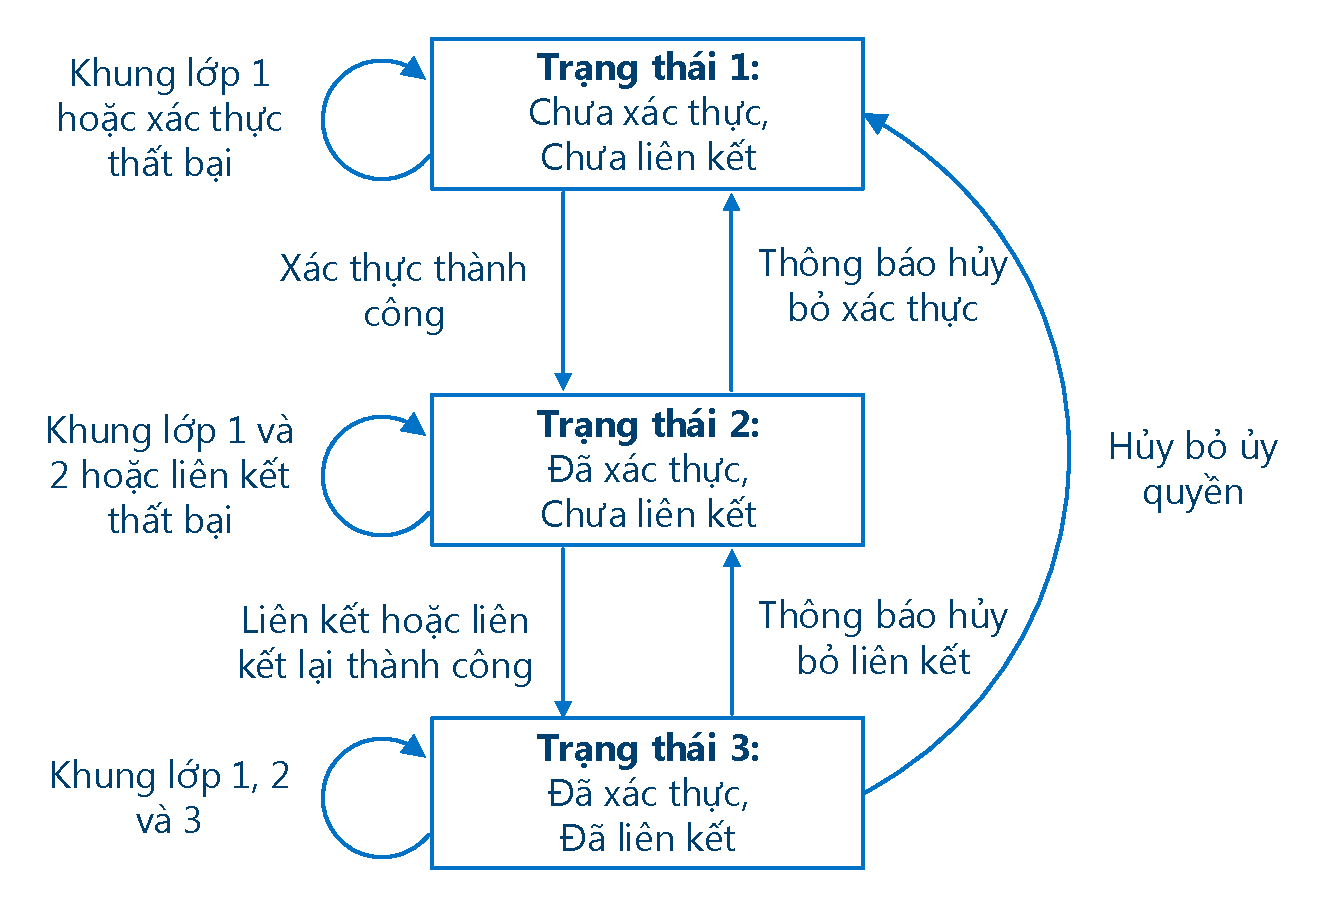
\includegraphics[width=1.0\textwidth]{authentication-and-association}
    \caption{
        \label{fig:authentication-and-association}
        Các giai đoạn xác thực và liên kết}% ~\cite{bidgoli2005hacking}
\end{figure}

\subsubsection*{\textit{a) Xác thực}}
\emph{Xác thực} là quá trình chứng minh nhận dạng của một STA đến STA khác hoặc AP. Trong xác thực hệ thống mở, tất cả các STA đều được xác thực mà không cần bất kỳ kiểm tra nào. Một STA A gửi một khung yêu cầu xác thực có chứa danh tính A, đến STA B. STA B trả lời với một khung cho biết sự công nhận, gửi tới A. Trong kiến trúc mạng khép kín, các STA phải biết SSID của AP để kết nối với AP. Xác thực khóa chia sẻ thì sử dụng một tiêu chuẩn thách đố và giải đố cùng với khóa bí mật chia sẻ. Trong phần sau, đồ án sẽ trình bày rõ hơn về một số tiêu chuẩn xác thực và mã hóa.

\begin{table}[!htbp]
\centering
\small
\setlength{\extrarowheight}{1pt}
\caption{\label{tab:management-class}Phân loại khung quản lý theo lớp}
\begin{tabular}{|c|p{10cm}|}
\hline
\textbf{Phân loại}     & \textbf{Tên khung}                            \\ \hline
\multirow{6}{*}{Lớp 1} & Probe Request                                 \\ \cline{2-2} 
                       & Probe Response                                \\ \cline{2-2} 
                       & Beacon                                        \\ \cline{2-2} 
                       & Authentication                                \\ \cline{2-2} 
                       & Deauthentication                              \\ \cline{2-2} 
                       & Announcement Traffic Indication Message (ATIM) \\ \hline
\multirow{3}{*}{Lớp 2} & Association Request/Response                  \\ \cline{2-2} 
                       & Reassociation Request/Response                \\ \cline{2-2} 
                       & Disassociation                                \\ \hline
Lớp 3                  & Deauthentication                              \\ \hline
\end{tabular}
\end{table}

\subsubsection*{\textit{b) Liên kết}}

Trao đổi dữ liệu giữa AP và STA chỉ có thể xảy ra khi STA đã được liên kết với AP trong mô hình mạng cơ sở hoặc với một STA khác ở mô hình mạng độc lập. Tất cả các AP truyền khung báo hiệu một số lần trong mỗi giây. Khung báo hiệu có chứa SSID, thời gian, khả năng, tốc độ và các thông tin khác. Liên kết có hai quá trình. Một STA mà chưa được xác thực và chưa liên kết sẽ lắng nghe khung báo hiệu để lựa chọn BSS mà nó muốn tham gia vào. STA và AP cùng nhau xác thực bằng cách trao đổi các khung xác thực. Khi đó, STA hiện đã được xác thực nhưng chưa được liên kết. Trong giai đoạn thứ hai, STA gửi khung yêu cầu liên kết và AP sẽ phản hồi lại một khung đáp ứng liên kết có chứa ID liên kết với STA. Khi đó, STA đã được xác thực và liên kết.

\subsection{Các tiêu chuẩn mã hóa}
Trong bảo mật mạng WiFi, người dùng thường chỉ quan tấm đến mật khẩu WiFi. Tuy nhiên cái thật sự quan trọng bên dưới chính là tiêu chuẩn mã hóa, việc lựa chọn tiêu chuẩn mã hóa phù hợp sẽ mang lại độ an toàn cao hơn cho mạng. Hầu hết các AP đều có khả năng cho phép một trong ba tiêu chuẩn mã hóa sau: Wired Equivalent Privacy (WEP), Wi-Fi Protected Access (WPA) hoặc Wi-Fi Protected Access II (WPA2).

Ngoài ra, chuẩn 802.11 cũng cho phép sử dụng hệ thống mở (Open System), tức là không sử dụng mã hóa các dữ liệu trong mạng. Tuy nhiên điều này tiềm ẩn nguy cơ về các vấn đề bảo mật, do vậy thường không được khuyến nghị sử dụng.

\subsubsection{WEP}
WEP là một giao thức mã hóa mặc định được giới thiệu lần đầu trong chuẩn IEEE 802.11 vào năm 1999. Nó sử dụng thuật toán mã dòng RC4 cho việc xác thực và mã hóa. Chuẩn này định nghĩa một khóa bí mật chia sẻ có độ dài 40 bit hoặc 104 bit. Khóa phải được quản trị viên nhập vào và cập nhật thủ công.

Khóa được kết hợp với một vector khởi tạo (IV) 24 bit nhằm mục đích tăng sức mạnh mã hóa. Tuy nhiên, kích thước IV nhỏ làm tăng khả năng khóa sẽ được sử dụng lại. Cùng với một số lỗ hỏng trong cơ chế xác thực, WEP ngày càng ít được sử dụng~\cite{guillaume2005wifi}.

\subsubsection{WPA}
Quá nhiều lỗ hỏng tồn tại trong WEP cho thấy nhu cầu cấp thiết cần một sự thay thế. Năm 2003, WiFi Alliance đã phát hành WPA như một tiêu chuẩn tạm thời, trong khi IEEE đang làm việc để phát triển một sự thay thế cao hơn, lâu dài hơn cho WEP. WPA có hai chế độ riêng cho người dùng doanh nghiệp và người dùng cá nhân. Chế độ doanh nghiệp, WPA-EAP, sử dụng xác thực 802.1x nghiêm ngặt hơn, với giao thức xác thực mở rộng EAP. Chế độ cá nhân, WPA-PSK, sử dụng các khóa được chia sẻ trước (pre-shared key) để thực hiện và quản lý đơn giản cho các khách hàng và văn phòng nhỏ. Chế độ doanh nghiệp yêu cầu sử dụng một máy chủ xác thực riêng~\cite{guillaume2005wifi}.

Mặc dù WPA cũng dựa trên thuật toán RC4, nhưng nó đã có một số cải tiến về mã hóa, cụ thể là việc sử dụng giao thức toàn vẹn khóa tạm thời (TKIP). Giao thức này bao gồm các tập chức năng để cải thiện bảo mật cho mạng WiFi: sử dụng khóa 256 bit, trộn khóa trên mỗi gói tin, tự động quảng bá các khóa được cập nhật, kiểm tra tính toàn vẹn thông điệp, kích thước IV lớn hơn (48 bit) và cơ chế giảm thiểu việc sử dụng lại IV.

WPA được thiết kế để tương thích ngược với WEP nhằm khuyến khích việc áp dụng nhanh chóng và dễ dàng. Chỉ với một bản cập nhật firmware mới, các thiết bị có thể hỗ trợ WPA với độ an toàn cao hơn.

\subsubsection{WPA2}
Tiêu chuẩn WPA2 hay còn gọi là 802.11i, được IEEE phê chuẩn vào năm 2004. Giống như WPA, WPA2 cũng cung cấp các chế độ dành cho doanh nghiệp và cá nhân. Mặc dù WPA2 còn tồn tại lỗ hỏng, nó vẫn được coi là chuẩn bảo mật mạng không dây an toàn nhất hiện có.

WPA2 thay thế thuật toán RC4 và TKIP bằng hai cơ chế mã hóa và xác thực mạnh hơn: chuẩn mã hóa nâng cao (AES) và giao thức CCMP. Ngoài ra để hỗ trợ tương thích ngược, WPA2 hỗ trợ TKIP như là một dự phòng nếu một thiết bị không thể hỗ trợ CCMP.

\subsection{Các tấn công trong mạng WiFi}
Phía sau sự tiện lợi của mạng WiFi, là khá nhiều mối đe dọa, đặc biệt là do các tấn công gây nên. Mục tiêu của chúng là những dữ liệu thông thường cho đến dữ liệu quan trọng, các tài khoản và dữ liệu bí mật khác~\cite{MEKHAZNIA2015172}.

\subsubsection{Giả mạo địa chỉ MAC}
Thuật ngữ "giả mạo địa chỉ MAC" trong ngữ cảnh này có nghĩa là kẻ tấn công thay đổi địa chỉ MAC mà nhà sản xuất gán vào card mạng thành địa chỉ khác. Việc giả mạo địa chỉ MAC khác với việc giả mạo địa chỉ IP, trong đó kẻ tấn công gửi dữ liệu từ một địa chỉ nguồn tùy ý và không mong đợi bất kỳ phản hồi nào đối với địa chỉ IP nguồn thật. Việc giả mạo địa chỉ MAC được mô tả chính xác hơn là giả mạo hoặc che dấu địa chỉ MAC vì kẻ tấn công không tạo ra dữ liệu với địa chỉ nguồn khác với địa chỉ của nó. Khi kẻ tấn công ghi đè địa chỉ MAC của mình, kẻ tấn công tiếp tục sử dụng card mạng không dây để truyền và nhận từ cùng một địa chỉ MAC nguồn~\cite{joshua2003detecting}. Tấn công này giúp kẻ tấn công vượt qua các cơ chế lọc địa chỉ MAC, một cơ chế xác thực thường được sử dụng ở các thiết bị AP.

\subsubsection{Tấn công từ chối dịch vụ}
\subsubsection*{\textit{a) Làm lụt khung xác thực/khung liên kết}}
Tấn công này cố áp đảo AP bằng các khung xác thực và khung liên kết. Để làm lụt các liên kết, kẻ tấn công sẽ giả mạo địa chỉ MAC của STA, sau đó liên tục cố liên kết với AP. Một trường hợp khác, kẻ tấn công sẽ thay thế địa chỉ MAC, giả mạo một lúc nhiều STA. Điều này làm cho bộ nhớ và khả năng xử lý của AP giảm, khiến AP từ chối STA ban đầu~\cite{scott2011known}.
	
\subsubsection*{\textit{b) Làm lụt khung hủy bỏ xác thực}}
Tấn công này hoạt động bằng cách khai thác điểm yếu cố hữu trong mạng không dây và thường được sử dụng như một phương pháp để bắt đầu tấn công giả mạo AP (Rogue Access Point - RAP). Kẻ tấn công gửi các khung hủy bỏ xác thực đến một STA đã kết nối với AP. STA nhận được khung hủy bỏ xác thực sẽ hủy bỏ liên kết với AP ngay khi có thể. Tấn công này hoạt động là vì các khung quản lý của AP không được mã hóa dẫn đến khung hủy bỏ xác thực được gửi đi tùy ý, bởi vậy rất dễ giả mạo. Tấn công này có thể tấn công trực tiếp lên AP, bằng cách gửi khung hủy bỏ xác thực đến địa chỉ MAC quảng bá với địa chỉ nguồn giả mạo là của AP~\cite{scott2011known}.

Các tấn công làm lụt có thể được phát hiện, vì một số lượng lớn khung hủy bỏ xác thực hoặc tương tự, sẽ tạo nên sự bất thường trong lưu lượng mạng.

\subsubsection{Man-in-the-middle}
Kẻ tấn công sử dụng tấn công Man-in-the-middle (MITM) để chặn bắt hoạt động trong mạng. Tấn công MITM bắt đầu với việc cấu hình một AP giả mạo (Rogue Access Point - RAP) để giả mạo AP gốc. Sau đó kẻ tấn công buộc STA kết nối với RAP bằng cách thực hiện tấn công từ chối dịch vụ lên AP gốc, hoặc bằng cách cung cấp tín hiệu mạnh hơn AP gốc. STA thường kết nối với AP có tín hiệu mạnh hơn. Để đánh lừa STA một cách chắc chắn, RAP thực hiện kết nối với các mạng khác để vẫn cung cấp kết nối Internet như bình thường. Nếu thành công, kẻ tấn công sẽ có thể có được quyền kiểm soát các kết nối mạng của STA. Với MITM, kẻ tấn công có thể giả mạo một trang web xác thực không dây để thu thập ID và mật khẩu; và thu thập các trang web, tên người dùng và mật khẩu được sử dụng trên các trang web. Tấn công này có thể được phát hiện đối với hệ thống mạng có ít AP, đối với hệ thống có nhiều AP đặt ở các vị trí xa nhau sẽ rất khó bảo vệ.

\subsubsection{Brute force WPS}
Thiết kế của Wi-Fi Protected Setup (WPS) có những nhược điểm cơ bản. Vì vậy, kẻ tấn công có thể lợi dụng những điểm yếu này để dò ra mã PIN chỉ trong vòng vài giờ.  Hình~\ref{fig:brute-force-wps-pin} là sơ đồ tấn công brute force mã PIN WPS~\cite{stefan2011brute}. Kẻ tấn công có thể nhận biết được liệu một phần của mã PIN là đúng hay không từ phản hồi của AP. Nếu kẻ tấn công nhận được thông báo EAP-NACK sau khi gửi M4, điều này có nghĩa là nửa đầu của mã PIN là chính xác. Nếu kẻ tấn công nhận được thông báo EAP-NACK sau khi gửi M6, điều đó có nghĩa là nửa cuối của mã PIN là chính xác. Mã PIN bao gồm 8 chữ số, do đó xác suất số PIN có giá trị là \(10^{8}\) hay là 100,000,000. Với phương thức tấn công này, số lần tấn công tối đa sẽ giảm xuống \(10^{4} + 10^{4}\), gấp 20,000 lần. Kể từ số thứ 8 của mã PIN, là tổng kiểm tra của các số từ 1 đến 7, do đó, cuộc tấn công sẽ giảm xuống \(10^{4} + 10^{3}\), là 11,000 lần.

\begin{figure}[H]
    \centering
    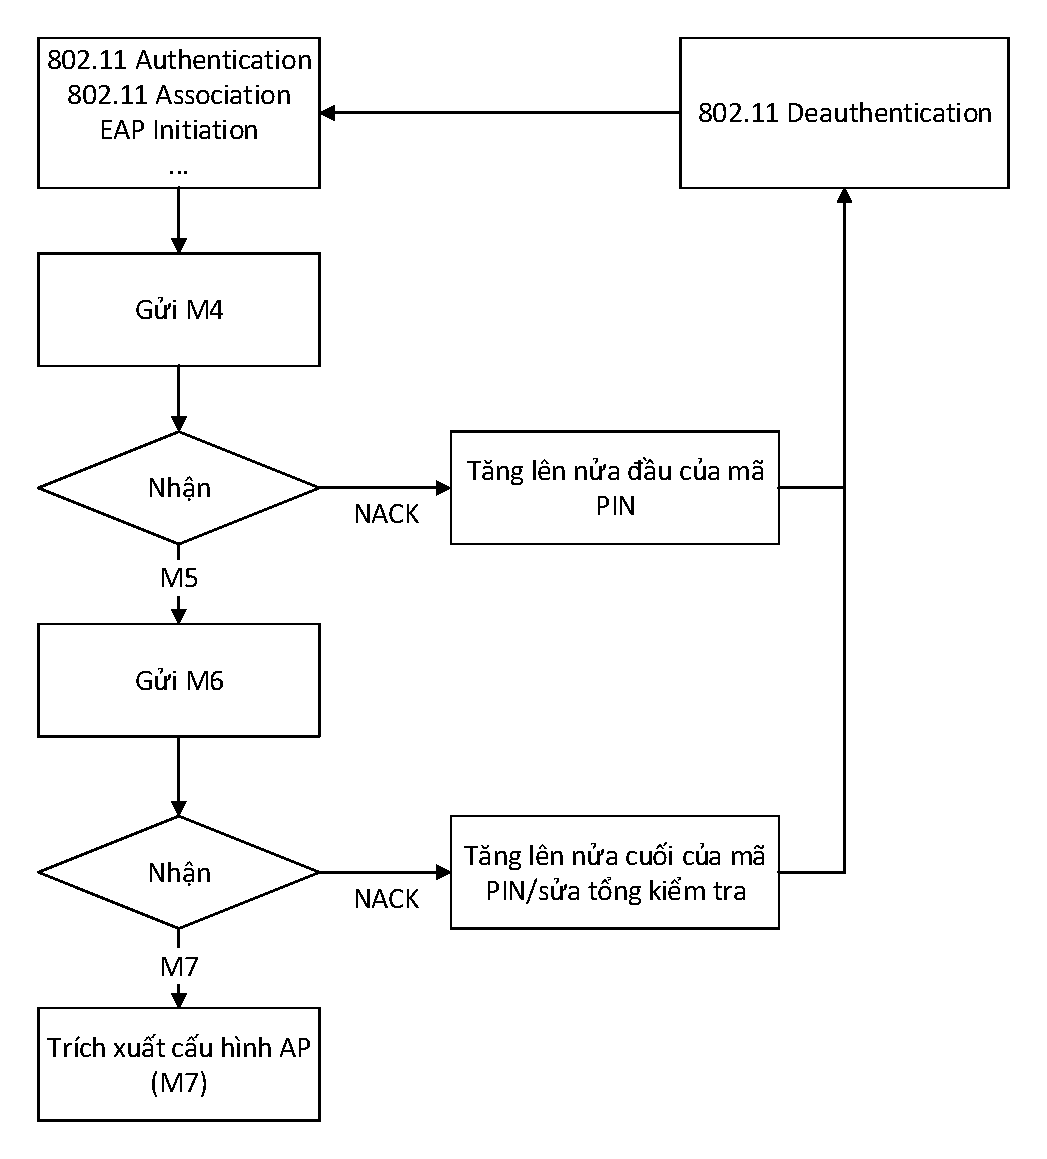
\includegraphics[width=0.85\textwidth]{brute-force-wps-pin}
    \caption{
        \label{fig:brute-force-wps-pin}
        Sơ đồ tấn công brute force mã PIN WPS}
\end{figure}

\begin{leftbar}
\noindent Ngoài những tấn công đặc trưng ở trên, người dùng trong mạng WiFi cũng có thể bị đe dọa bởi các tấn công tương tự như trong mạng có dây, như tấn công dò mật khẩu, tấn công quét cổng, phát tán mã độc, khai thác lỗ hỏng bảo mật. Trên đây là một số tấn công điển hình trong mạng WiFi, nhằm bảo vệ người dùng và phát hiện các mối đe dọa tiềm ẩn, mạng WiFi nên được thực hiện các giải pháp bảo mật, trong đó việc triển khai một hệ thống phát hiện xâm nhập là điều cần thiết.
\end{leftbar}

\section{Hệ thống phát hiện xâm nhập}
\subsection{Tổng quan}
\emph{Phát hiện xâm nhập} là quá trình giám sát các sự kiện xảy ra trong hệ thống máy tính hoặc mạng và phân tích các dấu hiệu của các sự cố có thể xảy ra, như là vi phạm hoặc đe dọa vi phạm chính sách bảo mật máy tính, các chính sách sử dụng được chấp nhận hoặc các tiêu chuẩn bảo mật trong thực tế. \emph{Ngăn chặn xâm nhập} là quá trình phát hiện xâm nhập và cố gắng ngăn chặn các sự cố có thể xảy ra. 

Theo tài liệu của Viện Tiêu chuẩn và Công nghệ Quốc gia Hoa Kỳ (NIST), hệ thống phát hiện xâm nhập (IDS) là các phần mềm tự động hóa quá trình phát hiện xâm nhập. Hệ thống ngăn chặn xâm nhập (IPS) là các phần mềm có tất cả chức năng của một hệ thống phát hiện xâm nhập và còn có thể cố gắng ngăn chặn các sự cố xảy ra nếu có thể~\cite{scarfone2007guide}. Như vậy, chức năng chính của IDS là tập trung vào việc xác định các sự cố có thể xảy ra, ghi lại thông tin về chúng, và báo cáo cho người quản trị. Trong phạm vi đồ án này, sẽ chỉ tập trung nghiên cứu về IDS, các chức năng chính và phương pháp phát hiện xâm nhập của nó.

\subsection{Các thành phần}
Các thành phần của một IDS bao gồm~\cite{scarfone2007guide}:

\begin{itemize}
\item \emph{Cảm biến và phần mềm đại diện (Sensor/Agent):} \tab Các cảm biến và phần mềm đại diện giám sát và phân tích các hoạt động. Các cảm biến thường được sử dụng để giám sát các mạng, và các phần mềm đại diện dùng để giám sát các máy tính đơn lẻ.

\item \emph{Máy chủ quản lý (Management Server):} \tab Một máy chủ quản lý là một thiết bị nhận các thông tin từ các cảm biến hoặc phần mềm đại diện và quản lý chúng. Nó cũng có thể thực hiện phân tích các thông tin nhận được và xác định các sự cố khi mà các cảm biến và phần mềm độc lập không thể.

\item \emph{Máy chủ cơ sở dữ liệu (Database Server):} \tab Một máy chủ cơ sở dữ liệu là một kho chứa cho các bản ghi thông tin sự kiện được ghi lại bởi các cảm biến, phần mềm đại diện, và các máy chủ quản lý.

\item \emph{Bảng điều khiển (Console):}  Một bảng điều khiển là một chương trình cung cấp một giao diện cho người sử dụng và quản trị viên của IDS. Bảng điều khiển thường được cài đặt lên các máy tính quản trị, phục vụ việc giám sát và quản trị IDS.
\end{itemize}

\subsection{Các chức năng chính}
Hiện nay có nhiều công nghệ IDS, được phân biệt chủ yếu bởi loại sự kiện mà chúng có thể nhận dạng và các phương pháp mà chúng sử dụng để xác định các sự cố. Ngoài chức năng chính là giám sát và phân tích các sự kiện để xác định các hoạt động không mong muốn. Hầu hết các công nghệ IDS đều có thể thực hiện các chức năng sau:

\begin{itemize}
\item \emph{Ghi lại các thông tin liên quan đến các sự kiện quan sát được:} \tab Thông tin có thể ghi lại cục bộ hoặc được gửi đến các hệ thống riêng biệt như máy chủ nhật ký tập trung, các giải pháp quản lý sự kiện an ninh (SIEM) và các hệ thống quản lý doanh nghiệp.

\item \emph{Thông báo cho các quản trị viên bảo mật về các sự kiện quan trọng được quan sát:} \tab Các thông báo này gọi chung là cảnh báo (alert). Chúng được gửi đến quản trị viên thông qua thư điện tử, thông điệp cảnh báo trên giao diện bảng điều khiển IDS, giao thức SMTP, thông điệp syslog và các chương trình và script do người dùng định nghĩa. Các thông báo này thường chỉ bao gồm thông tin cơ bản về sự kiện, quản trị viên cần truy cập IDS để biết thêm thông tin.

\item \emph{Xuất báo cáo:} \tab Báo cáo tóm tắt các sự kiện được theo dõi hoặc cung cấp chi tiết về các sự kiện cụ thể được quan tâm.
\end{itemize}

\subsection{Các phương pháp phát hiện phổ biến}
Các công nghệ IDS sử dụng nhiều phương pháp để phát hiện xâm nhập. Sau đây đồ án sẽ trình bày về các phương pháp phát hiện xâm nhập phổ biến bao gồm: \emph{phát hiện dựa trên chữ ký (signature-based)}, \emph{phát hiện dựa trên sự bất thường (anomaly-based)}, và \emph{phân tích giao thức có trạng thái (stateful protocol analysis)}~\cite{scarfone2007guide}. Hầu hết các sản phẩm IDS sử dụng nhiều phương pháp phát hiện, hoạt động độc lập hoặc kết hợp với nhau, để gia tăng phạm vi và độ chính xác cho việc phát hiện xâm nhập.

\subsubsection{Phát hiện dựa trên chữ ký}
\emph{Chữ ký} là một mẫu tương ứng với một mối đe dọa đã biết. \emph{Phát hiện dựa trên chữ ký} là quá trình so sánh các chữ ký với các sự kiện quan sát được để xác định các sự cố có thể xảy ra. Ưu điểm của phương pháp này là cho hiệu quả cao khi phát hiện các mối đe dọa đã biết. Tuy nhiên, nó không thể phát hiện các mối đe dọa chưa biết trước đó, các mối đe dọa sử dụng kỹ thuật lẩn trốn, và các biến thể của các mối đe dọa đã biết.

Phát hiện dựa trên chữ ký là một phương pháp phát hiện đơn giản nhất, vì nó chỉ thực hiện các hoạt động so sánh chuỗi. Các công nghệ phát hiện dựa trên chữ ký không có hiểu biết nhiều về các giao thức mạng hoặc ứng dụng, nên không thể theo dõi và hiểu được trạng thái của các liên lạc phức tạp. Chúng cũng thiếu khả năng ghi nhớ các yêu cầu trước đó khi xử lý yêu cầu hiện tại. Hạn chế này ngăn cản việc phát hiện các cuộc tấn công gồm nhiều sự kiện nhưng không có sự kiện nào có dấu hiệu rõ ràng về một cuộc tấn công.

\subsubsection{Phát hiện dựa trên sự bất thường}
\emph{Phát hiện dựa trên sự bất thường} là quá trình so sánh các định nghĩa về hoạt động được coi là bình thường với các sự kiện quan sát được để xác định độ lệch đáng kể. IDS sử dụng phương pháp phát hiện dựa trên sự bất thường có các hồ sơ biểu diễn các hành vi bình thường của người dùng, máy chủ, kết nối mạng hoặc ứng dụng. Các hồ sơ này được phát triển bằng cách giám sát các đặc tính của hoạt động điển hình trong một khoảng thời gian. Ví dụ, một hồ sơ cho một mạng cho thấy rằng hoạt động web trung bình chiếm 13\% băng thông mạng trong một ngày làm việc bình thường. IDS sau đó sử dụng các phương pháp thống kê để so sánh các đặc tính của hoạt động hiện tại với các ngưỡng có liên quan đến hồ sơ, chẳng hạn như phát hiện khi hoạt động web có băng thông cao hơn trung bình đáng kể và cảnh báo sự bất thường đến một quản trị viên. Các hồ sơ có thể được phát triển cho nhiều thuộc tính hành vi, chẳng hạn như số lượng thư điện tử được gửi bởi người dùng, số lần đăng nhập không thành công vào máy chủ và mức độ sử dụng bộ vi xử lý của máy chủ trong một khoảng thời gian nhất định.

Lợi ích chính của phương pháp phát hiện dựa trên sự bất thường là chúng rất hiệu quả khi phát hiện các mối đe dọa chưa biết trước đó. Một hồ sơ khởi tạo được sinh trong một khoảng thời gian định kỳ, còn được gọi là huấn luyện định kỳ. Hồ sơ cho phát hiện dựa trên sự bất thường có thể là hồ sơ tĩnh hoặc hồ sơ động. Hồ sơ tĩnh sau khi được sinh ra sẽ không thể thay đổi, trừ khi tạo thêm một hồ sơ mới. Hồ sơ động được điều chỉnh liên tục khi các sự kiện bổ sung được quan sát.

Phương pháp phát hiện dựa trên sự bất thường có nhược điểm là khả năng phát hiện dương tính giả cao. Ví dụ, các hoạt động bảo trì, sao lưu thường tạo ra lưu lượng truyền tải lớn, có thể bị cảnh báo như một hành vi bất thường.

\subsubsection{Phân tích giao thức có trạng thái}
\emph{Phân tích giao thức có trạng thái} là quá trình so sánh các hồ sơ đã xác định trước các sự kiện quan sát được để xác định độ lệch. Các hồ sơ này chứa các định nghĩa chung về hoạt động hợp lệ của giao thức được cho phép cho mỗi trạng thái của giao thức. Không giống như phát hiện dựa trên sự bất thường, sử dụng các hồ sơ máy chủ hoặc mạng cụ thể, phân tích giao thức có trạng thái dựa vào các hồ sơ chung được phát triển của nhà cung cấp để chỉ định cách mà các giao thức cụ thể nên và không nên sử dụng. Thuật ngữ "có trạng thái" trong phân tích giao thức có trạng thái có nghĩa là IDS có khả năng hiểu và theo dõi trạng thái của các giao thức ở lớp mạng, lớp vận chuyển và lớp ứng dụng mà có khái niệm về trạng thái.

Phân tích giao thức có trạng thái có thể xác định các câu lệnh có trình tự không mong muốn, chẳng hạn như các câu lệnh sử dụng lặp đi lặp lại hoặc sử dụng một câu lệnh mà không cần sử dụng câu lệnh ban đầu mà nó phụ thuộc. Một tính năng theo dõi trạng thái khác của phân tích giao thức có trạng thái là đối với các giao thức xác thực, IDS dựa vào đó để xác định các hoạt động khác nhau có thể chấp nhận đối với nhiều lớp người dùng hoặc người dùng cụ thể.

Phương pháp phân tích giao thức có trạng thái sử dụng các mô hình giao thức, thường dựa vào các tiêu chuẩn giao thức từ các nhà cung cấp phần mềm và các cơ quan phát hành tiêu chuẩn (ví dụ RFC của IETF). Nhiều tiêu chuẩn không giải thích đầy đủ chi tiết của giao thức, tạo nên những biến thể khi thực hiện giao thức. Ngoài ra, đối với các giao thức độc quyền, thông tin chi tiết về các giao thức thường không có sẵn, làm cho công nghệ IDS khó thực hiện phân tích chính xác và toàn diện.

Hạn chế chính của phương pháp phân tích giao thức có trạng thái là chúng cần rất nhiều tài nguyên do sự phức tạp của việc phân tích và chi phí liên quan trong việc thực hiện theo dõi trạng thái cho nhiều phiên đồng thời. Một vấn đề nghiêm trọng khác là các phương pháp phân tích giao thức có trạng thái không thể phát hiện các cuộc tấn công không vi phạm các đặc tính của các hành vi giao thức thông thường được chấp nhận, chẳng hạn như thực hiện nhiều hành động hợp lệ trong một khoảng thời gian ngắn để gây ra sự từ chối dịch vụ.

\subsection{Phân loại}
Hệ thống phát hiện xâm nhập có thể chia làm hai loại chính là hệ thống phát hiện xâm nhập mạng (NIDS) và hệ thống phát hiện xâm nhập máy chủ (HIDS). Mỗi loại có những chức năng và ưu nhược điểm riêng.

\subsubsection{Hệ thống phát hiện xâm nhập mạng}
\emph{Hệ thống phát hiện xâm nhập mạng} hoạt động như một thiết bị độc lập trên mạng. Nó thường được đặt ở các phân đoạn mạng hoặc các điểm kết nối giữa các vùng mạng khác nhau. Nhờ đó nó có thể giám sát lưu lượng mạng từ nhiều nguồn khác nhau trong vùng mạng đó. NIDS có thể là một thiết bị phần cứng hoặc phần mềm. Về cấu trúc thì NIDS thường bao gồm một tập hợp các cảm biến (sensor) được đặt ở các điểm khác nhau trong mạng. Các cảm biến này sẽ thực hiện giám sát lưu lượng mạng, thực hiện phân tích cục bộ lưu lượng mạng đó và báo cáo về cho trung tâm quản lý (Center Management Console). Snort, Suricata là những NIDS điển hình.

Ưu điểm của NIDS là có thể quản lý được cả một phân đoạn mạng gồm nhiều máy, với một mạng được thiết kế tốt, nó mang lại sự hiệu quả về mặt chi phí đáng kể. Vì khả năng hoạt động ở chế độ lắng nghe bị động, có thể cài đặt và bảo trì NIDS đơn giản, không ảnh hưởng tới mạng, cung cấp sự bảo vệ "trong suốt" đối với cả người dùng và kẻ tấn công.

Bên cạnh đó, NIDS có thể gặp những khó khăn trong việc xử lý tất cả các gói tin trong một mạng có kích thước lớn và mật độ lưu lượng cao, khả năng NIDS bị quá tải và không thể phát hiện được các tấn công là rất lớn. NIDS cũng biểu lộ nhược điểm khi làm việc với dữ liệu phân mảnh hay mã hóa, nó không thể phân tích được các thông tin đã bị mã hóa, và các dạng tấn công phân mảnh dữ liệu.

\subsubsection{Hệ thống phát hiện xâm nhập máy chủ}
\emph{Hệ thống phát hiện xâm nhập máy chủ} hoạt động trên một máy tính đơn lẻ. HIDS sẽ sử dụng các tài nguyên của máy chủ đó để theo dõi lưu lượng truy cập và phát hiện các cuộc tấn công nếu có. Bằng cách này HIDS có thể theo dõi được tất cả các hoạt động trên máy tính đó như tập tin nhật ký và những lưu lượng mạng ra vào nó. Ngoài ra HIDS còn theo dõi hệ điều hành, các sự kiện, các thông báo lỗi của máy chủ. Không phải hầu hết các cuộc tấn công đều thông qua mạng, nên không phải lúc nào NIDS cũng có thể phát hiện được cuộc tấn công trên một máy tính. Ví dụ, kẻ tấn công có quyền truy cập vật lý, từ đó có thể xâm nhập vào máy tính đó mà không cần tạo ra bất cứ lưu lượng mạng nào. Một ưu điểm của HIDS so với NIDS đó là nó có thể phát hiện các dạng tấn công phân mảnh dữ liệu. Bởi vậy nên HIDS thường được cài đặt trên các trên các máy chủ quan trọng của tổ chức, các máy chủ trong vùng DMZ. Một số HIDS phổ biến đó là OSSEC, Proventia Desktop.

Ngoài khả năng phát hiện các dạng tấn công phân mảnh dữ liệu, HIDS cũng có thể làm việc với dữ liệu mã hóa. Tuy nhiên, do phải cài đặt phần mềm giám sát (agent) lên các máy tính cần bảo vệ, nên nó đặt ra khá nhiều vấn đề cho công tác quản lý, cấu hình, cập nhật. HIDS cũng chiếm một phần tài nguyên hệ thống, và phụ thuộc nhiều vào hệ điều hành bên dưới nó, nên cần có những thiết lập tối ưu để mang lại hiệu quả phát hiện cao nhất.

\section{Hệ thống phát hiện xâm nhập mạng không dây}
\subsection{Giới thiệu}
Các hệ thống phát hiện xâm nhập được dùng để nhận diện mối đe dọa tới hệ thống mạng và máy tính bằng cách thu thập và phân tích dữ liệu. IDS thường chỉ được sử dụng cho hệ thống và mạng có dây. Trong thời gian gần đây, IDS đã được phát triển để sử dụng cho mạng không dây, được gọi là hệ thống phát hiện xâm nhập mạng không dây (Wireless Intrusion Detection System - WIDS). Những WIDS này có thể giám sát và phân tích hoạt động của người dùng và hệ thống, nhận biết các dạng tấn công đã biết, các hành vi bất thường trong mạng và các vi phạm chính sách cho mạng không dây. Các WIDS thu thập tất cả các liên lạc không dây cục bộ và tạo ra các cảnh báo dựa trên các chữ ký được xác định trước hoặc các bất thường trong lưu lượng truy cập.

WIDS cũng giống với một IDS chuẩn cho mạng có dây, nhưng thường yêu cầu về triển khai cũng như một số đặc tả chức năng riêng biệt để phát hiện xâm nhập cho mạng không dây.

\subsection{Các thành phần và kiến trúc}

\subsubsection{Các thành phần chính}
Các thành phần chính của WIDS giống với NIDS, bao gồm: bảng điều khiển, máy chủ cơ sở dữ liệu (tùy chọn), máy chủ quản lý, và cảm biến~\cite{scarfone2007guide}. Tất cả các thành phần (ngoại trừ các cảm biến) có chung chức năng cho tất cả các loại IDS. Cảm biến không dây thực hiện vai trò cơ bản giống như đối với cảm biến NIDS, nhưng chức năng rất khác bởi vì có nhiều phức tạp trong việc giám sát liên lạc không dây. Một cảm biến không dây chỉ có thể giám sát một kênh riêng lẻ tại một thời điểm, do đó có thể bỏ lỡ những hành vi trái phép trên các kênh khác. Vì vậy cảm biến sẽ thay đổi kênh thường xuyên, kỹ thuật này gọi là quét kênh (channel scanning), để có thể giám sát mỗi kênh một số lần trong mỗi giây.

Cảm biến không dây thông thường có một số dạng:
\begin{itemize}
\item \emph{Cảm biến riêng:} \tab Một cảm biến riêng là một thiết bị thực hiện các chức năng WIDS nhưng sẽ không hỗ trợ truyền dữ liệu từ nguồn tới đích. Nó sẽ hoạt động hoàn toàn bị động, một số chúng thực hiện phân tích lưu lượng, một số khác thì chuyển tiếp lưu lượng đến máy chủ quản lý để phân tích. Cảm biến riêng có thể được triển khai cố định tại các vị trí cụ thể hoặc di động.

\item \emph{Cảm biến đi kèm với một AP:} \tab Cảm biến đi kèm thường có khả năng phát hiện ít nghiêm ngặt như một cảm biến riêng vì AP cần phân chia thời gian giữa việc cung cấp truy cập mạng và giám sát trên nhiều kênh để phát hiện hành vi trái phép. Cảm biến này phù hợp cho việc giám sát ở một dải tần và kênh đơn lẻ.

\item \emph{Cảm biến đi kèm với một bộ chuyển mạch không dây:} \tab Bộ chuyển mạch không dây được dùng để quản lý và giám sát các thiết bị không dây. Tuy nhiên nó không cung cấp khả năng phát hiện mạnh như cảm biến đi kèm AP và cảm biến riêng.
\end{itemize}

\subsubsection{Kiến trúc mạng}
Các thành phần WIDS thường được kết nối với nhau thông qua mạng có dây, thể hiện giống như Hình~\ref{fig:wids-architecture}. Một mạng quản lý tách biệt hoặc mạng chuẩn của tổ chức có thể sử dụng cho các liên lạc giữa các thành phần của WIDS.

\begin{figure}[!h]
    \centering
    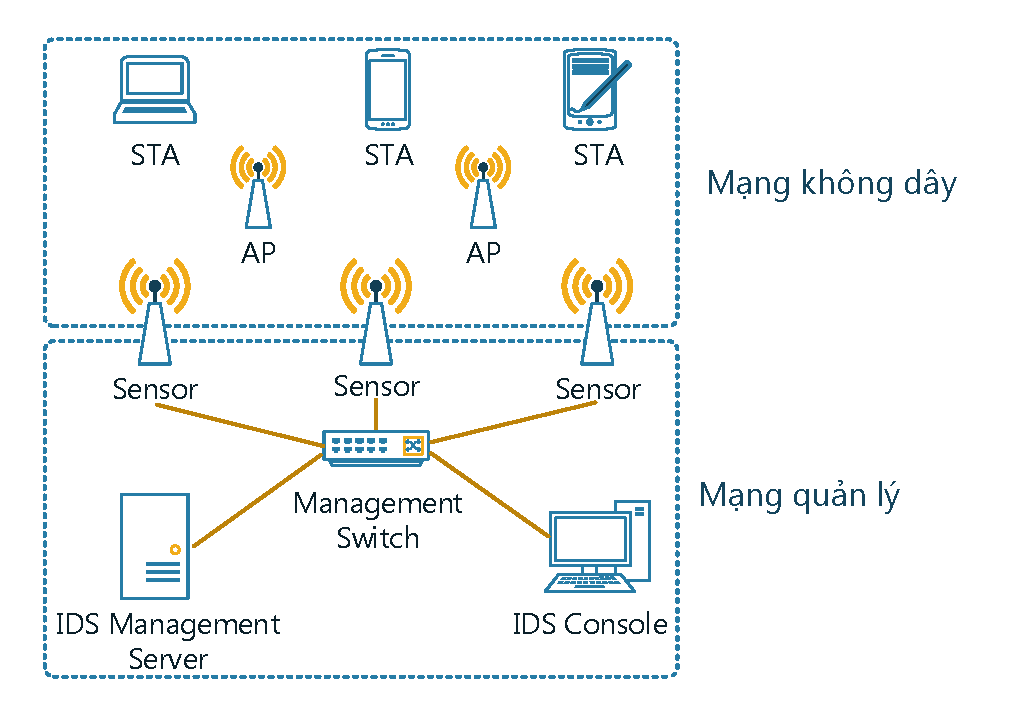
\includegraphics[width=1.0\textwidth]{wids-architecture}
    \caption{
        \label{fig:wids-architecture}
        Kiến trúc chung của WIDS}
\end{figure}

\subsection{Các tính năng bảo mật}

\subsubsection{Thu thập thông tin}
Hầu hết WIDS có thể thu thập các thông tin trên thiết bị không dây. Điển hình là nhận dạng các thiết bị trong mạng, bao gồm các AP, các STA, dựa trên BSSID và địa chỉ MAC của card mạng không dây. Ngoài ra, hầu hết các cảm biến cũng theo dõi các mạng, đánh dấu mạng nào được ủy quyền, mạng nào là mạng bên ngoài tổ chức hoặc các mạng giả mạo.

\subsubsection{Ghi nhật ký}
Các WIDS thường thực hiện mở rộng việc ghi nhật ký dữ liệu liên quan để phát hiện các sự kiện an ninh. Những dữ liệu này có thể được sử dụng để xác nhận tính hợp lệ của các cảnh báo, để điều tra các sự cố, và các mối liên hệ giữa IDS và các nguồn nhật ký khác. Các loại dữ liệu thường được ghi nhật ký bởi WIDS bao gồm:

\begin{itemize}
\item Nhãn thời gian
\item Loại sự kiện hoặc cảnh báo
\item Mức độ ưu tiên hoặc nghiêm trọng
\item Địa chỉ MAC nguồn (nhà sản xuất nào sẽ được nhận dạng)
\item Số thứ tự kênh
\item ID của cảm biến mà quan sát sự kiện
\item Hành động ngăn chặn đã thực hiện (nếu có tính năng ngăn chặn xâm nhập)
\end{itemize}

\subsubsection{Phát hiện xâm nhập}
Cũng giống như một hệ thống phát hiện xâm nhập thông thường, WIDS có thể phát hiện các tấn công, cấu hình sai, và vi phạm chính sách ở mức giao thức mạng không dây. WIDS thường không kiểm tra các truyền thông ở các mức cao (ví dụ như địa chỉ IP, dữ liệu lớp ứng dụng). Một số sản phẩm thực hiện chỉ kỹ thuật phát hiện dựa trên chữ ký, trong khi số khác sử dụng kết hợp các kỹ thuật phát hiện dựa trên chữ ký, phát hiện dựa trên hành vi bất thường, và phân tích giao thức có trạng thái. Dưới đây là các loại sự kiện thường được phát hiện bởi cảm biến WIDS~\cite{scarfone2007guide}:

\begin{itemize}
\item \emph{Mạng không dây hoặc thiết bị không dây trái phép:} \tab Thông qua khả năng thu thập thông tin, hầu hết các cảm biến WIDS có thể phát hiện các AP giả mạo, các STA trái phép, và cả các mạng trái phép.

\item \emph{Các thiết bị kém an toàn:} \tab Các WIDS có thể phát hiện các cấu hình sai, cũng như sử dụng các giao thức yếu. Điều này được thực hiện bằng cách xác định những sai khác từ các chính sách cụ thể của tổ chức cho các cài đặt mã hóa, xác thực, SSID và kênh.

\item \emph{Mẫu hành vi sử dụng bất thường:} \tab Một số cảm biến có thể sử dụng phương pháp phát hiện dựa trên hành vi bất thường để phát hiện các mẫu sử dụng bất thường. Những mẫu sử dụng bất thường điển hình là những nỗ lực tham gia vào mạng thất bại trong một khoảng thời gian, hoặc các hoạt động mạng ngoài giờ.

\item \emph{Sử dụng các công cụ quét mạng:} \tab Các công cụ quét mạng được sử dụng để nhận dạng các điểm yếu và mất an toàn của mạng không dây. WIDS chỉ có thể phát hiện việc sử dụng các công cụ quét chủ động, tức chúng có phát sinh lưu lượng mạng. Chúng không thể phát hiện việc sử dụng các cảm biến mà đơn giản chỉ giám sát và phân tích lưu lượng quan sát được.

\item \emph{Các điều kiện và tấn công từ chối dịch vụ:} \tab Tấn công từ chối dịch vụ có thể được phát hiện thông qua phương pháp phân tích trạng thái giao thức hoặc hành vi bất thường. Các tấn công từ chối dịch vụ được phát hiện thường được theo dõi trong suốt một thời gian và cảnh báo khi mà đạt đến một giá trị ngưỡng.

\item \emph{Các tấn công giả mạo và Man-in-the-middle:} \tab Một vài cảm biến WIDS có thể phát hiện khi mà một thiết bị cố gắng để giả mạo danh tính của thiết bị khác.
\end{itemize}

Hầu hết WIDS có thể xác định vị trí vật lý của một mối đe dọa được phát hiện bằng cách tính toán ước lượng khoảng cách gần đúng.

Mặc dù WIDS cung cấp khả năng phát hiện mạnh mẽ những chúng có một số hạn chế đáng kể. Một số vấn đề quan trọng như là không thể phát hiện được một số cuộc tấn công không dây, dễ bị trộm cắp, và không thể chịu được các cuộc tấn công chống lại chính WIDS. Cụ thể là tấn công không dây như giám sát bị động thì WIDS không thể phát hiện được. Thêm nữa, một cảm biến WIDS cũng dễ dàng bị tấn công, điển hình là tấn công từ chối dịch vụ sẽ làm gián đoạn chức năng của cảm biến.

\subsubsection{Khả năng quản lý}
Hầu hết sản phẩm WIDS có khả năng quản lý đơn giản. Sau khi lựa chọn sản phẩm WIDS, quản trị viên cần thiết kế một kiến trúc mạng, thực hiện kiểm tra các thành phần, đảm bảo an ninh cho các thành phần, và sau đó triển khai chúng. Vận hành và bảo trì WIDS gần giống như đối với NIDS. Bảng điều khiển WIDS cung cấp tính năng như quản lý, giám sát, phân tích, và báo cáo. Việc triển khai các WIDS có thể yêu cầu phải ngừng hoạt động mạng không dây trong một thời gian ngắn để nâng cấp hoặc cài đặt phần mềm IDS.

\section{Các hệ thống đã được phát triển}
Trong phần này, đồ án sẽ khảo sát về một số hệ thống WIDS đã được phát triển, bao gồm các sản phẩm WIDS từ các hãng nổi tiếng như Cisco, Netscout và một số dự án WIDS mã nguồn mở điển hình.

\subsection{Cisco Unified Wireless Network}
Cisco Unified Wireless Network (CUWN) là một giải pháp của Cisco giành cho doanh nghiệp. Nó cung cấp sự an toàn, khả năng mở rộng, và tiết kiệm chi phí cho mạng không dây doanh nghiệp~\cite{cisco2015enterprise}. CUWN gồm các thành phần chính là Aironet access points (AP), Wireless LAN controller (WLC), Cisco Prime Infrastructure và Mobility Services Engine (MSE); trong đó, WLC đóng vai trò là một thành phần phát hiện xâm nhập cho các tấn công trong mạng không dây. WLC thực hiện phân tích lưu lượng không dây của các AP đã kết nối và báo cáo khi phát hiện tấn công đến các WLC khác hoặc Wireless Control System (WCS). Ngoài ra, WLC cũng thực hiện phân tích bổ sung lưu lượng mạng có dây như một NIDS. Các tập tin chữ ký của WLC được bao gồm trong các bản phát hành phần mềm, nó cũng cho phép cập nhật độc lập từng tập tin, hoặc tự định nghĩa các chữ ký mới. Bảng dưới đây (Bảng~\ref{tab:cisco-wlc-signature}) là danh sách các chữ ký chuẩn của Cisco WLC~\cite{cisco2015enterprise}.

\begin{table}[h!]
\centering
\small
\setlength{\extrarowheight}{1pt}
\caption{\label{tab:cisco-wlc-signature}Các chữ ký chuẩn của Cisco WLC}
\begin{tabular}{|c|p{3.9cm}|c|p{6.8cm}|}
\hline
\multicolumn{1}{|l|}{\textbf{STT}} & \textbf{Tên}          & \textbf{Kiểu khung} & \textbf{Mô tả}                                 \\ \hline
1                                  & Bcast deauth          & Management          & Broadcast Deauthentication Frame               \\ \hline
2                                  & NULL probe resp 1     & Management          & NULL Probe Response - Zero length SSID element \\ \hline
3                                  & NULL probe resp 2     & Management          & NULL Probe Response - No SSID element          \\ \hline
4                                  & Assoc flood           & Management          & Association Request flood                      \\ \hline
5                                  & Auth flood            & Management          & Authentication Request flood                   \\ \hline
6                                  & Reassoc flood         & Management          & Reassociation Request flood                    \\ \hline
7                                  & Broadcast Probe flood & Management          & Broadcast Probe Request flood                  \\ \hline
8                                  & Disassoc flood        & Management          & Disassociation flood                           \\ \hline
9                                  & Deauth flood          & Management          & Deauthentication flood                         \\ \hline
10                                 & Reserved mgmt 7       & Management          & Reserved management sub-type 7                 \\ \hline
11                                 & Reserved mgmt F       & Management          & Reserved management sub-type F                 \\ \hline
12                                 & EAPOL flood           & Data                & EAPOL Flood Attack                             \\ \hline
13                                 & NetStumbler 3.2.0     & Data                & NetStumbler 3.2.0                              \\ \hline
14                                 & NetStumbler 3.2.3     & Data                & NetStumbler 3.2.3                              \\ \hline
15                                 & NetStumbler 3.3.0     & Data                & NetStumbler 3.3.0                              \\ \hline
16                                 & NetStumbler generic   & Data                & NetStumbler                                    \\ \hline
17                                 & Wellenreiter          & Management          & Wellenreiter                                   \\ \hline
\end{tabular}
\end{table}

Hơn thế, CUWN cũng cung cấp thành phần tích hợp Adaptive Wireless Intrusion Prevention System (wIPS) với khả năng ngăn chặn các cuộc tấn công trong mạng không dây. CUWN có thể gửi cảnh báo qua SNMP tới hệ thống quản lý WCS, và gửi thư điện tử qua SMTP đến nhà quản trị.

Tuy nhiên, so với thị trường như nước ta thì giá thành của giải pháp CUWN vẫn khá cao. Qua khảo sát, có thể thấy được chi phí để triển khai một giải pháp CUWN cơ bản của Cisco khoảng trên 8000 USD, bao gồm 1 Cisco Wireless Controler hỗ trợ cho 12 Access Point với giá 4000 USD~\cite{router2017airwlc}, 2 Access Point giá 1000 USD~\cite{router2017airap} cho hệ thống chỉ hỗ trợ 5 Access Point. Ngoài ra hệ thống này cũng cần có nhân viên quản trị được đào tạo để cài đặt, cấu hình, quản lý. Vì vậy, Cisco cũng cung cấp các khóa học để đào tạo và tổ chức thi các chứng chỉ quản trị cho hệ thống này.

\subsection{AirMagnet Enterprise}

Bên cạnh CUWN của Cisco, hãng bảo mật Netscout cũng đưa ra một giải pháp WIDS/IPS có tên là AirMagnet Enterprise. Kiến trúc của WIDS/IPS này gồm một hoặc nhiều máy chủ quản lý, được gọi là AirMagnet Enterprise Server (AME), và nhiều cảm biến WIDS/IPS, được gọi là AirMagnet Sensors và AirMagnet Spectrum Sensors. Hình~\ref{fig:ame-architect} mô tả kiến trúc của một hệ thống AirMagnet Enterprise điển hình.

\begin{figure}[H]
    \centering
    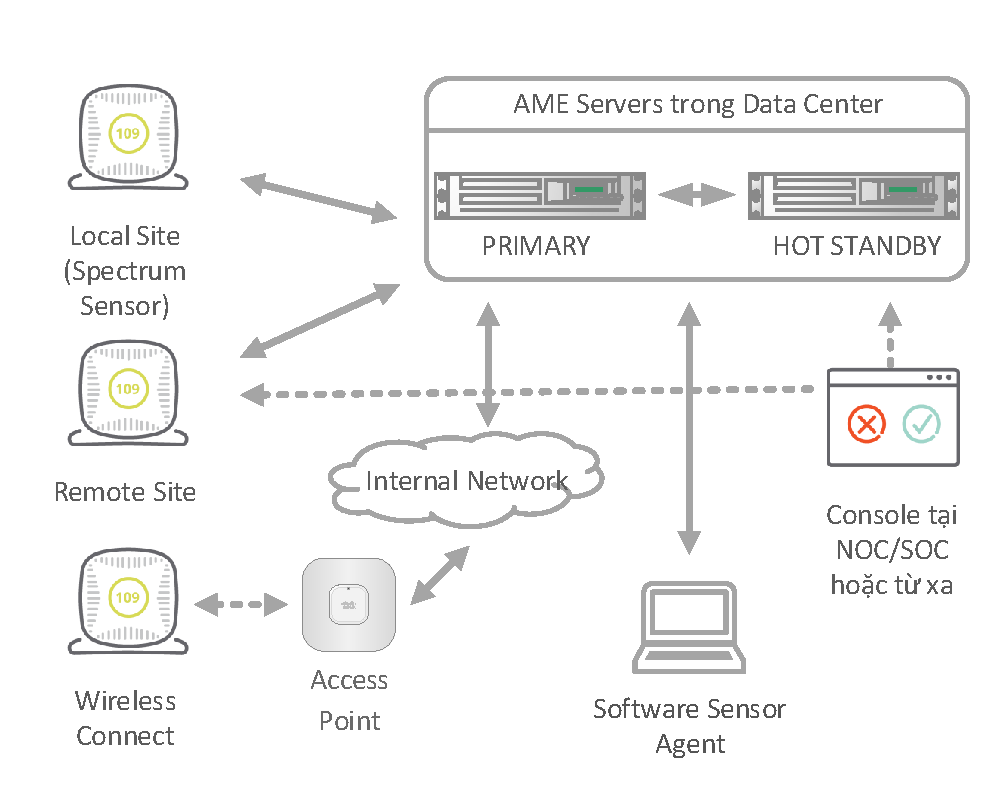
\includegraphics[width=0.8\textwidth]{ame-architect}
    \caption{
        \label{fig:ame-architect}
        Kiến trúc của AirMagnet Enterprise}
\end{figure}

Hầu hết WIDS/IPS đều có khả năng phát hiện tấn công mạng không dây cơ bản nhất như phát hiện ra AP giả mạo và các thiết bị STA trái phép. AirMagnet Enterprise không phải là ngoại lệ. Nó cũng cung cấp nhiều khả năng phát hiện tấn công tiên tiến, bao gồm phát hiện các tấn công từ chối dịch vụ và các tấn công giả mạo, cũng như lập bản đồ vị trí vật lý của các thiết bị STA và AP. AirMagnet Enterprise không cung cấp khả năng phát hiện tấn công xác thực và nỗ lực phá mã, đây là tính năng mà khá ít hệ thống WIDS/IPS hỗ trợ~\cite{karen2016fluke}.

Ưu điểm đáng lưu ý của AirMagnet Enterprise là cung cấp khả năng thu thập dữ liệu và báo cáo rất mạnh mẽ, nó có thể ghi lại tất cả các sự kiện cơ bản và thu thập các gói dữ liệu. Nó cũng hỗ trợ báo cáo theo các tiêu chuẩn tuân thủ bảo mật như PCI-DSS, HIPAA~\cite{karen2016fluke}.

\begin{leftbar}
\noindent Qua khảo sát hai sản phẩm khá nổi tiếng ở trên, có thể thấy chúng đều có khả năng giám sát và phát hiện các cuộc tấn công trong mạng không dây, lưu trữ các thông tin liên quan đến cuộc tấn công vào cơ sở dữ liệu, gửi cảnh báo qua SNMP, SMTP. Tuy nhiên, các giải pháp này đều chủ yếu giành cho đối tượng khách hàng doanh nghiệp với giá thành khá cao, thị trường doanh nghiệp nhỏ, trường học, hay quán cà phê vẫn đang bỏ ngỏ. Trong các phần dưới dây, đồ án sẽ trình bày về một số WIDS nguồn mở, điển hình là Snort Wireless và Kismet Wireless.
\end{leftbar}

\subsection{Snort Wireless}
Snort là một NIDS đã quá phổ biến. Vì vậy vào năm 2004, cộng đồng mã nguồn mở đã phát triển một dự án gọi là Snort Wireless, nhằm mở rộng khả năng của Snort để phát hiện các tấn công trong mạng không dây. Nó hoàn toàn tương thích ngược với Snort 2.0.x và thêm một số tính năng bổ sung. Snort Wireless đặc tả các luật thông qua một quy tắc luật mới, gọi là giao thức \emph{wifi}, có thể phát hiện hầu hết các tấn công trong mạng không dây như tấn công giả mạo, các công cụ quét mạng như Netstumbler~\cite{caswell2005nessus}. Bảng~\ref{tab:snort-wireless-rule-options} là danh sách các tùy chọn trong luật của Snort Wireless~\cite{valli2004wireless} .

\newgeometry{a4paper,left=3.5cm,right=2cm,top=3cm,bottom=3cm}
\headsep=0pt

\begin{table}[H]
\centering
\small
\setlength{\extrarowheight}{1pt}
\caption{\label{tab:snort-wireless-rule-options}Các tùy chọn trong luật của Snort Wireless}
\begin{tabular}{|p{4cm}|p{10.5cm}|}
\hline
\textbf{Tùy chọn} & \textbf{Mô tả}                                          \\ \hline
frame\_control    & kiểm tra trường điều khiển toàn bộ khung                \\ \hline
type              & kiểm tra kiểu khung của 802.11                          \\ \hline
stype             & kiểm tra kiểu khung phụ của 802.11                      \\ \hline
from\_ds          & kiểm tra cờ điều khiển khung từ hệ thống phân phối      \\ \hline
to\_ds            & kiểm tra cờ điều khiển khung đến hệ thống phân phối     \\ \hline
more\_frags       & kiểm tra cờ điều khiển trong các khung \emph{more fragment}    \\ \hline
retry             & kiểm tra cờ điều khiển trong khung \emph{retry}                \\ \hline
pwr\_mgmt         & kiểm tra cờ điều khiển trong các khung \emph{power management} \\ \hline
more\_data        & kiểm tra cờ điều khiển trong khung dữ liệu              \\ \hline
wep               & kiểm tra cờ điều khiển trong khung \emph{wep}                  \\ \hline
order             & kiểm tra cờ điều khiển thứ tự khung                      \\ \hline
duration\_id      & kiểm tra các trường \emph{duration-id} của khung                     \\ \hline
bssid             & kiểm tra trường BSSID của khung                                 \\ \hline
seqnum            & kiểm tra trường \emph{sequence number} của khung                \\ \hline
fragnum           & kiểm tra trường \emph{fragment number} của khung      \\ \hline
addr4             & kiểm tra trường địa chỉ thứ tư  của khung           \\ \hline
ssid              & kiểm tra trường SSID của khung                    \\ \hline
\end{tabular}
\end{table}

Luật của Snort Wireless có cú pháp như sau:

\begin{lstlisting}
<action> wifi <src mac> -> <dst mac> (<rule options>)
\end{lstlisting}

Cụ thể hơn, gói cài đặt Snort Wireless cũng cung cấp một số luật mặc định trong tập tin \emph{rules/wifi.rules}~\cite{caswell2005nessus}:\\

\begin{lstlisting}
alert wifi any -> any (msg:"Association Request"; stype:STYPE_ASSOCREQ;)
alert wifi any -> any (msg:"Association Response";stype:STYPE_ASSOCRESP;)
alert wifi any -> any (msg:"Reassociation Request"; stype:STYPE_REASSOC_ REQ;)
alert wifi any -> any (msg:"Reassociation Response"; stype:STYPE_REASSO C_RESP;)
alert wifi any -> any (msg:"Probe Request"; stype:STYPE_PROBEREQ;)
alert wifi any -> any (msg:"Probe Response"; stype:STYPE_PROBERESP;)
alert wifi any -> any (msg:"Beacon"; stype:STYPE_BEACON;)
\end{lstlisting}

\restoregeometry
\newgeometry{a4paper,left=3.5cm,right=2cm,top=3cm,bottom=3cm}
\headsep=0pt

\begin{lstlisting}
alert wifi any -> any (msg:"ATIM"; stype:STYPE_ATIM;)
alert wifi any -> any (msg:"Disassociation"; stype:STYPE_DISASSOC;)
alert wifi any -> any (msg:"Authentication"; stype:STYPE_AUTH;)
alert wifi any -> any (msg:"Deauthentication"; stype:STYPE_DEAUTH;)
\end{lstlisting}

Snort Wireless thực sự là một dự án WIDS tiềm năng, tuy nhiên hiện nay nó đã không còn được phát triển, dù chưa có thông báo chính thức nào. Các mã nguồn cài đặt và thư viện liên quan đều đã lỗi thời. Vì lý do này, trong hệ thống WIDS sẽ đề xuất, đồ án sẽ không lựa chọn Snort Wireless.

\subsection{Quadrant Information Security}
Quadrant Information Security cũng đưa ra một giải pháp WIDS miễn phí dựa trên các phần mềm mã nguồn mở~\cite{champ2014building}. Hệ thống này sử dụng một máy tính gồm một card mạng có dây và hai card mạng không dây. Card mạng có dây được kết nối ra Internet và chuyển tiếp các lưu lượng của AP ra Internet, card mạng không dây thứ nhất được dùng để giả lập AP thông qua phần mềm \emph{hostapd}, card mạng không dây còn lại đóng vai trò như một cảm biến WIDS để giám sát các tấn công lớp 2 từ bên ngoài mạng vào AP được giả lập. Snort được cài đặt như một NIDS, có thể giám sát lưu lượng không dây của AP. Kismet đảm nhiệm vai trò WIDS với cài đặt theo kiến trúc tiêu chuẩn, cả thành phần Kismet drone và Kismet server trên cùng máy tính. Như vậy, có thể thấy hệ thống WIDS này rất đa năng, có thể phát hiện được các tấn công bên trong và bên ngoài mạng không dây.

Đây là một thử nghiệm tuyệt vời về ưu điểm của các phần mềm mã nguồn mở, mang lại một giải pháp có giá thành thấp hơn rất nhiều so với các sản phẩm của các hãng như Cisco, Netscout. Tuy nhiên, nó cũng có nhược điểm lớn về triển khai, đó là kích thước của máy tính lớn hơn nhiều so với một AP, nên không thể đặt ở những vị trí treo tường hay ngoài trời, những nơi thực sự cần đặt cảm biến không dây. Hơn nữa, điện năng tiêu thụ và chi phí bảo trì phần cứng cũng cần được quan tâm, bởi vì một máy tính thông thường sẽ không phù hợp cho việc chạy liên tục trong một thời gian dài.

\restoregeometry

\section{Kismet Wireless}
\subsection{Giới thiệu}
Kismet là một ứng dụng phân tích mạng mã nguồn mở. Nó xác định các mạng bằng cách thụ động thu thập các gói tin. Kismet có thể phát hiện  các SSID ẩn và các mạng không quảng bá thông qua lưu lượng dữ liệu. Kismet có thể chạy với bất kỳ card mạng không dây nào hỗ trợ chế độ giám sát, và có thể chặn bắt lưu lượng 802.11b, 802.11a, 802.11g, và 802.11n. Ngoài ra, Kismet cũng có kiến trúc mở rộng, cho phép thêm các giao thức ngoài 802.11 để giải mã được~\cite{mike2016kismet}.

Các phần mở rộng của Kismet có thể thực hiện hầu hết mọi thứ giống như tiến trình Kismet có thể thực hiện. Phần mở rộng cho phép mở rộng khả năng ghi nhật ký, thêm các cảnh báo IDS, định nghĩa các nguồn thu mới và thêm các tính năng mới vào Kismet UI.

Kismet cung cấp tính năng WIDS cả có trạng thái và phi trạng thái cho các tấn công lên lớp 2 và lớp 3 của mạng không dây. Hiện tại tính năng phát hiện xâm nhập cho lớp 3 vẫn đang được phát triển. Kismet phát hiện tấn công và tạo cảnh báo dựa trên chữ ký - \emph{fingerprint} (cho các các tấn công đơn lẻ cụ thể) và dựa trên xu hướng/phân tích trạng thái - \emph{trend/stateful} (cho các tấn công sử dụng khung thăm dò bất thường, tấn công làm lụt khung hủy bỏ liên kết).

Kismet có thể tích hợp với các công cụ khác sử dụng \emph{tun/tap export} để cung cập một giao diện mạng ảo của lưu lượng không dây; các công cụ như Packet-o-Matic và Snort có thể sử dụng những dữ liệu đã xuất này để thực hiện các chức năng IDS bổ sung.\\ \\ \\

\subsection{Kiến trúc của Kismet}
Kismet được cấu tạo với thành phần Kismet drone làm nó trở thành một hệ thống WIDS phân tán. Kiến trúc của Kismet bao gồm:

\begin{itemize}
\item \emph{Kismet drone:} thu thập dữ liệu trong mạng và gửi chúng tới Kismet server.
\item \emph{Kismet server:} xử lý các dữ liệu.
\item \emph{Kismet client:} hiển thị các kết quả xử lý dữ liệu đã thu thập được.
\end{itemize}

\subsection{Các cảnh báo của Kismet}
Kismet mặc định cho phép 1 cảnh báo mỗi giây và tối đa 5 cảnh báo mỗi phút. Kismet hỗ trợ phát hiện hơn 20 loại tấn công trong mạng không dây~\cite{mike2016kismet}. Các cảnh báo điển hình được liệt kê trong Bảng~\ref{tab:cac-canh-bao-cua-kismet}.

\newgeometry{a4paper,left=3.5cm,right=2cm,top=3cm,bottom=2cm}
\headsep=0pt

\begin{table}[!htbp]
\centering
\small
\setlength{\extrarowheight}{0.2pt}
\caption{\label{tab:cac-canh-bao-cua-kismet}Các cảnh báo của Kismet}
\begin{tabular}{|p{4.4cm}|p{2.3cm}|p{7.3cm}|}
\hline
\textbf{Tên cảnh báo}                                                         & \textbf{Loại}  & \textbf{Mô tả}                                                                                                                                                                                                                                                                                                       \\ \hline
AIRJACKSSID                                                                   & Fingerprint    & Các công cụ tấn công mạng 802.11 trước đây, như Airjack, thường đặt SSID mặc định là \emph{airjack} khi khởi động lên.                                                                                                                                                                                                         \\ \hline
APSPOOF                                                                       & Fingerprint    & Nếu một khung báo hiệu hoặc đáp ứng thăm dò cho SSID đó được nhìn thấy từ một địa chỉ MAC không nằm trong danh sách MAC hợp lệ, cảnh báo này sẽ được đưa ra. Điều này có thể được sử dụng để phát hiện các AP xung đột, AP giả mạo, hoặc các tấn công như Karma/Airbase, những tấn công mà đáp ứng lại tất cả khung yêu cầu thăm dò. \\ \hline
BSSTIMESTAMP                                                                  & Trend/Stateful & Một nhãn thời gian có số thứ tự không hợp lệ/ngoài phạm vi có thể cho thấy sự giả mạo AP.                                                                                                                                                                                                                            \\ \hline
CHANCHANGE                                                                    & Trend/Stateful & Một AP đã được phát hiện trước đó, thay đổi kênh có thể cho thấy là tấn công giả mạo.                                                                                                                                                                                                                                \\ \hline
CRYPTODROP                                                                    & Trend/Stateful & Một AP giả mạo với ít tùy chọn mã hóa, ít bảo mật hơn có thể đánh lừa STA kết nối và thu thập thông tin xác thực.                                                                                                                                                                                          \\ \hline
\begin{tabular}[c]{@{}l@{}}DEAUTHFLOOD\\BCASTDISCON\end{tabular}             & Trend/Stateful & Bằng cách giả mạo các khung hủy bỏ liên kết và hủy bỏ xác thực, kẻ tấn công có thể ngắt kết nối các STA khỏi mạng, gây ra một tấn công từ chối dịch vụ, kéo dài cho tới khi kẻ tấn công tiếp tục gửi các khung đó.                                                                                               \\ \hline
DHCPCLIENTID                                                                  & Fingerprint    & Một STA gửi gói tin DHCP DISCOVER có chứa một Client-ID tag (Tag 61) không trùng khớp với địa chỉ MAC nguồn của gói tin, có thể đang thực hiện một tấn công từ chối dịch vụ DHCP để làm cạn kiệt DHCP Pool.                                                                                                       \\ \hline
DHCPCONFLICT                                                                  & Trend/Stateful & Các STA nhận một địa chỉ DHCP và tiếp tục sử dụng một địa chỉ IP khác có thể cho thấy một sự cấu hình sai hoặc là STA giả mạo.                                                                                                                                                                                 \\ \hline
DISASSOCTRAFFIC                                                               & Trend/Stateful & Một STA đã hủy bỏ liên kết khỏi một mạng không nên ngay lập tức tiếp tục trao đổi dữ liệu. Đây có thể cho thấy một STA giả mạo cố gắng tiêm các dữ liệu không hợp lệ vào mạng, hoặc có thể cho thấy một STA đang là nạn nhân của một tấn công từ chối dịch vụ.                                              \\ \hline
\begin{tabular}[c]{@{}l@{}}DISCONCODEINVALID\\DEAUTHCODEINVALID\end{tabular} & Fingerprint    & Đặc tả kỹ thuật 802.11 định nghĩa các giá trị hợp lệ \textit{reason code} cho các sự kiện ngắt kết nối và hủy bỏ xác thực.    \\ \hline
\end{tabular}
\end{table}

% Please add the following required packages to your document preamble:
% \usepackage[normalem]{ulem}
% \useunder{\uline}{\ul}{}
\begin{table}[!htbp]
\centering
\small
\setlength{\extrarowheight}{1pt}
%\caption{\label{tab:cac-canh-bao-cua-kismet}Các cảnh báo của Kismet}
\begin{tabular}{|p{4.4cm}|p{2.3cm}|p{7.3cm}|}
\hline
%\textbf{Tên cảnh báo}                                                         & \textbf{Loại}  & \textbf{Mô tả}                                                                                                                                                                                                                                                                                                       \\ \hline
                                                                      &     & Nhiều STA và AP đã báo cáo lại các xử lý sai của \textit{reason code} không hợp lệ.                                                                                                               \\ \hline
\begin{tabular}[c]{@{}l@{}}DHCPNAMECHANGE\\DHCPOSCHANGE\end{tabular}         & Trend/Stateful & Giao thức cấu hình DHCP cho phép các STA tùy ý đặt \emph{hostname} và \emph{DHCP client vendor/operating system} trong gói tin DHCP Discover. Những giá trị này nên chỉ thay đổi khi STA đã thực sự thay đổi (ví dụ như hệ thống khởi động song song). Việc thay đổi giá trị có thể cho thấy một STA giả mạo/tấn công giả mạo địa chỉ MAC.    \\ \hline
LONGSSID                                                                      & Fingerprint    & Đặc tả kỹ thuật 802.11 cho phép tối đa 32 byte cho SSID. Các SSID quá kích thước là dấu hiệu của một cuộc tấn công cố gắng để khai thác lỗ hỏng bảo mật trên một số trình điều khiển.                                                                                                                                          \\ \hline
LUCENTTEST                                                                    & Fingerprint    & Các thẻ Old Lucent Orinoco trong các chế độ quét kiểm tra nhất định sẽ tạo ra các gói tin có thể nhận dạng được.                                                                                                                                                                                                     \\ \hline
MSFBCOMSSID                                                                   & Fingerprint    & Một số phiên bản của trình điều khiển Windows Broadcom không xử lý đúng các trường SSID dài hơn đặc tả kỹ thuật 802.11, dẫn đến hệ thống bị thỏa hiệp và thực thi mã lệnh. Lỗ hỏng bảo mật này có thể khai thác bằng Metasploit framework.                                                                              \\ \hline
MSFDLINKRATE                                                                  & Fingerprint    & Một số phiên bản của trình điều khiển Windows D-Link không xử lý đúng các trường rate hợp lệ quá dài, dẫn đến hệ thống bị thỏa hiệp và thực thi mã lệnh. Lỗ hỏng bảo mật này có thể khai thác bằng Metasploit framework.                                                                                               \\ \hline
MSFNETGEARBEACON                                                              & Fingerprint    & Một số phiên bản của trình điều khiển Windows Netgear không xử lý đúng các khung báo hiệu quá kích cỡ, dẫn đến hệ thống bị thỏa hiệp và thực thi mã lệnh. Lỗ hỏng bảo mật này có thể khai thác bằng Metasploit framework.                                                                                                \\ \hline
NETSTUMBLER                                                                   & Fingerprint    & Các phiên bản cũ hơn của Netstumbler (3.22, 3.23, 3.30) trong một điều kiện nhất định, sẽ tạo ra các gói tin cụ thể.                                                                                                                                                                                                 \\ \hline
NULLPROBERESP                                                                 & Fingerprint    & Các khung đáp ứng thăm dò với thành phần SSID IE tag có chiều dài bằng 0 có thể làm các thẻ cũ hơn (prism2, orinoco, airport-classic) bị lỗi.                                                                                                                                                                       \\ \hline
PROBENOJOIN                                                                   & Trend/Stateful & Các công cụ quét chủ động như Netstumbler liên tục gửi các khung yêu cầu thăm dò mạng nhưng không bao giờ tham gia bất cứ mạng nào gửi đáp ứng lại.                                                                                                                                                                         \\ \hline
\end{tabular}
\end{table}

\restoregeometry%


\section{Snort}
\subsection{Giới thiệu}
Snort là một hệ thống phát hiện và phòng chống xâm nhập mạng mã nguồn mở được phát triển bởi Sourcefire, được Cisco mua lại từ năm 2013. Kết hợp việc kiểm tra chữ ký, hành vi bất thường và phân tích giao thức có trạng thái, Snort đã được triển khai rộng khắp trên toàn thế giới. Với hơn 4 triệu lượt tải về và hơn 500.000 lượt người dùng đăng ký, Snort đã trở thành tiêu chuẩn của hệ thống phát hiện và ngăn chặn xâm nhập~\cite{snort2017documents}.

Snort có thể chạy theo ba chế độ:
\begin{itemize}
\item \emph{Chế độ lắng nghe (Sniffer mode):} ở chế độ này, Snort sẽ đọc cái gói tin trong mạng và hiển thị chúng theo một luồng liên tục trên bảng điều khiển hoặc màn hình.
\item \emph{Chế độ ghi lại gói tin (Packet Logger mode):} ghi lại các gói tin vào đĩa cứng.
\item \emph{Chế độ phát hiện xâm nhập mạng (NIDS mode):} thực hiện phát hiện và phân tích trên lưu lượng mạng. Đây là chế độ phức tạp nhất và có thể cấu hình.
\end{itemize}

\subsection{Kiến trúc của Snort}
Kiến trúc của Snort gồm 4 thành phần cơ bản sau~\cite{caswell2007snort}:

\begin{itemize}
\item Thành phần lắng nghe, giải mã gói tin (Packet Sniffer).
\item Thành phần tiền xử lý (Preprocessor).
\item Thành phần phát hiện (Detection Engine).
\item Thành phần cảnh báo/ghi nhật ký (Alert/Logging).\\
\end{itemize}

Hình~\ref{fig:snort-architecture} cung cấp một cái nhìn trực quan về kiến trúc và quá trình xử lý của Snort, luồng xử lý tuần tự từ trái sang phải.

\begin{figure}[H]
    \centering
    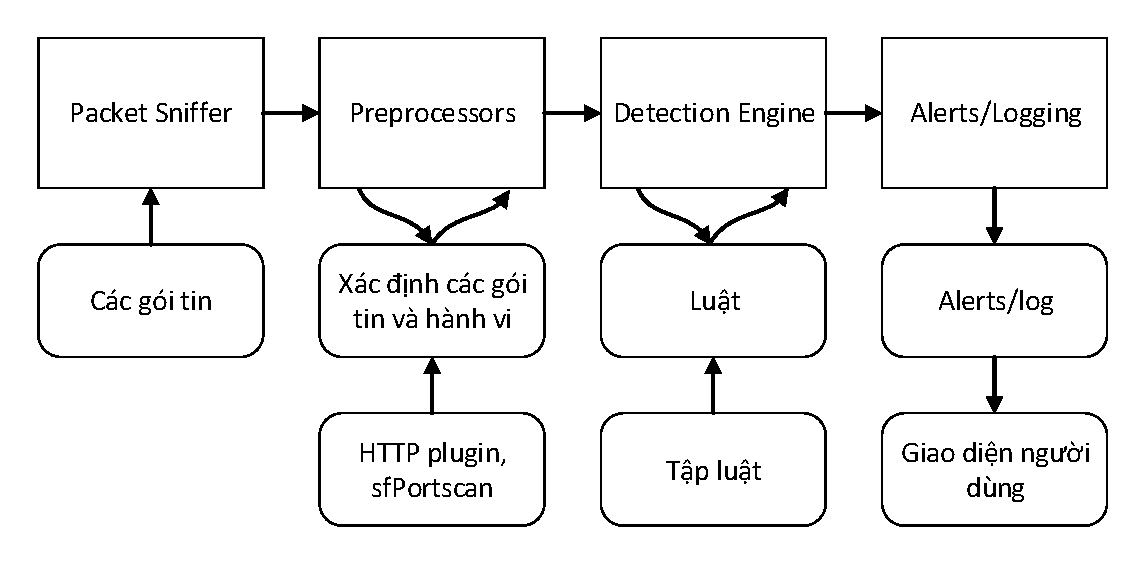
\includegraphics[width=1.0\textwidth]{snort-architecture}
    \caption{
        \label{fig:snort-architecture}
        Kiến trúc của Snort}
\end{figure}

\emph{Thành phần lắng nghe, giải mã gói tin} là một thiết bị phần cứng hoặc phần mềm được đặt trong mạng. Chức năng của nó là phân tích các giao thức thành thông tin mà con người có thể đọc và hiểu được, hỗ trợ giải mã các giao thức khác nhau bao gồm IP, ICMP, TCP, UDP thành dữ liệu các lớp trên.

\emph{Thành phần tiền xử lý} cho phép phân tích cú pháp dữ liệu theo những cách khác nhau. Một số mô-đun hỗ trợ như sau: Frag3 - mô-đun chống phân mảnh gói tin IP, sfPortscan - mô-đun được thiết kế chống lại các cuộc do thám, như quét cổng, xác định dịch vụ, xác định hệ điều hành, Stream5 - mô-đun tái gộp các gói tin ở tầng TCP. Ở thời điểm hiện tại Snort có 24 mô-đun tiền xử lý~\cite{caswell2007snort}.

\emph{Thành phần phát hiện} là một phần của hệ thống phát hiện xâm nhập dựa trên chữ ký. Nó chịu trách nhiệm lấy dữ liệu từ thành phần tiền xử lý và kiểm tra chúng thông qua các luật. Nếu các luật đó khớp với dữ liệu trong gói tin, nó sẽ được gửi tới hệ thống cảnh báo, nếu không nó sẽ bị bỏ qua. Luật là phần quan trọng nhất của Snort, các cú pháp luật của Snort sẽ được giới thiệu thêm ở mục tiếp theo.

Thành phần cuối cùng là \emph{cảnh báo/ghi nhật ký}. Nếu dữ liệu khớp với một luật trong thành phần phát hiện, một cảnh báo sẽ được đưa ra. Các cảnh báo có thể được gửi đến các tập tin nhật ký, gửi qua mạng thông qua SNMP, SMTP hoặc cũng có thể lưu trữ vào cơ sở dữ liệu như MySQL. Giống như thành phần tiền xử lý, chức năng này được cấu hình trong tập tin cấu hình của Snort, có thể chỉ định cảnh báo và ghi lại trong tập tin cấu hình nếu muốn kích hoạt. Snort cũng hỗ trợ nhiều phần mở rộng giúp người quản trị nhận các cảnh báo cũng như phân tích các dữ liệu một cách trực quan. Bảng~\ref{tab:snort-addons} là danh sách một số phần mở rộng cho Snort.

\begin{table}[!htbp]
\centering
\small
\setlength{\extrarowheight}{0.2pt}
\caption{\label{tab:snort-addons}Một số phần mở rộng hỗ trợ cho Snort}
\begin{tabular}{|p{4cm}|p{10.5cm}|}
\hline
\textbf{Tên phần mở rộng}                 & \textbf{Mô tả}                                                                                                                                          \\ \hline
ACID                                      & ACID được biết như một phần mở rộng phân tích cú pháp nhật ký dựa trên PHP, cung cấp khả năng tìm kiếm và là một giao diện phân tích nhật ký của Snort. \\ \hline
SGUIL                                    & Một nền tảng web cung cấp tính năng giám sát và phân tích nhật ký cho Snort.                                                                            \\ \hline
Oinkmaster                             & Một Pert script giúp cập nhật các luật của Snort và có thể đánh dấu những luật không muốn sau mỗi lần cập nhật.                                         \\ \hline
IDS Policy Manager               & Một giao diện quản lý dành cho Windows XP.                                                                                                              \\ \hline
SnortSnarf                               & Một chương trình viết bằng Perl giúp tạo và cung cấp các bản báo cáo log gần đây một cách tổng hợp dưới dạng HTML.                                      \\ \hline
Swatch                                     & Một công cụ giám sát nhật ký hệ thống theo thời gian thực và gửi cảnh báo bằng email.                                                                   \\ \hline
BASE                                      & Một giao diện web cho Snort, cung cấp khả năng truy vấn và cảnh báo cho Snort.                                                                          \\ \hline
\end{tabular}
\end{table}

\subsection{Tập luật}
Snort sử dụng một ngôn ngữ mô tả tập luật đơn giản, nhưng cũng khá hiệu quả và mạnh mẽ. Hầu hết các luật của Snort được viết trên một dòng, và có thể mở rộng thành nhiều dòng bằng ký tự gạch chéo ngược "\textbackslash " ở cuối mỗi dòng. Luật của Snort bao gồm 2 phần: tiêu đề luật (rule header) và tùy chọn luật (rule option)~\cite{snort2017documents}.

\subsubsection{Tiêu đề luật}
\emph{Rule header} gồm 4 phần: Rule action, Protocol, Src/Dst và Port.

\begin{itemize}
\item \emph{Rule action:} Rule action sẽ nói cho Snort biết sẽ làm gì khi tìm thấy gói tin phù hợp với các luật đã định sẵn. Có 5 hành động là: \emph{Alert} - cảnh báo, \emph{Log} - ghi nhật ký, \emph{Pass} - cho qua, \emph{Active} - kích hoạt, \emph{Dynamic} - duy trì trạng thái nhàn rỗi đến khi được kích hoạt.
\item \emph{Protocol:} chỉ ra giao thức mà Snort sẽ phân tích: TCP, UDP, ICMP và IP.
\item \emph{IP address:} địa chỉ IP của nơi đi và nơi đến của 1 gói tin. Ví dụ: \emph{192.168.1.1 \tab 192.168.2.1} cho biết địa chỉ nguồn là 192.168.1.1 và địa chỉ đích là 192.168.2.1.
\item \emph{Port:} số hiệu cổng dịch vụ mà Snort sẽ phân tích. Ví dụ: 80 của HTTP, 22 của SSH.
\end{itemize}

\subsubsection{Các tùy chọn luật}
\emph{Rule option} là trung tâm của việc phát hiện xâm nhập. Nội dung của nó chứa các dấu hiệu để xác định một cuộc xâm nhập. Rule option nằm ngay sau Rule header và được bao bọc bởi dấu ngoặc đơn "\(()\)". Tất cả Rule option được ngăn cách nhau bởi dấu chấm phẩy "\(;\)", phần đối số sẽ được phân cách nhau bởi dấu hau chấm "\(:\)".

Có bốn loại Rule option chính bao gồm:
\begin{itemize}
\item \emph{General:} gồm các tùy chọn cung cấp thông tin về luật đó nhưng không có bất cứ ảnh hưởng nào trong quá trình phát hiện.
\item \emph{Payload:} gồm các tùy chọn liên quan đến phần tải của gói tin.
\item \emph{Non-payload:} gồm các tùy chọn không liên quan đến phần tải của gói tin.
\item \emph{Post-detection:} gồm các tùy chọn áp dụng một luật cụ thể sau khi một luật được bỏ qua.
\end{itemize}

\subsubsection*{\textit{a) General}}

\begin{itemize}
\item \emph{Msg:} gán thêm một chuỗi văn bản vào nhật ký và cảnh báo. Chuỗi đó được đặt trong dấu ngoặc kép \(" "\). Ví dụ: \emph{msg: "Hello World"}.
\item \emph{Reference:} dùng khi muốn tham chiếu thông tin từ một hệ thống khác trên internet.
\item \emph{Sid:} được dùng để xác định duy nhất một luật trong Snort.
\item \emph{Rev:} được sử dụng để định danh các sửa đổi trong luật của Snort, thường dùng để phân biệt các phiên bản luật khác nhau.
\item \emph{Classtype:} được dùng để phân loại các hình thức tấn công kèm theo độ ưu tiên của loại tấn công đó và được định nghĩa trong tập tin \emph{classification.config}.
\item \emph{Priority:} được sử dụng để gán độ nghiêm trọng của một luật.
\end{itemize}

\subsubsection*{\textit{b) Payload}}

\begin{itemize}
\item \emph{Content:} cho phép tìm kiếm các chuỗi cụ thể trong phần tải của gói tin (payload) và kích hoạt các cảnh báo dựa trên các dữ liệu đó. Nội dung có thể ở dạng nhị phân hoặc ASCII. Ví dụ: \emph{content: "GET"}
\item \emph{Nocase:} kết hợp với từ khóa content để tìm kiếm chuỗi mà không phân biệt hoa thường.
\item \emph{Rawbyte:} cho phép các luật xem các gói dữ liệu thô chưa được giải mã.
\item \emph{Depth:} dùng để xác định khoảng cách bao xa mà luật đó sẽ tìm tới, tối thiểu là 1 và tối đa là 65535. Nó được dùng với từ khóa content để giới hạn nội dung tìm kiếm.
\item \emph{Offset:} dùng để xác định điểm bắt đầu tìm kiếm, cho phép giá trị từ \emph{-65535} đến \emph{65535}.
\item \emph{Distance:} được sử dụng trong trường hợp muốn bỏ qua bao nhiêu byte từ nội dung tìm kiếm trước đó.
\item \emph{Within:} được dùng để đảm bảo rằng có nhiều nhất N byte giữa các mẫu nội dung tìm kiếm.
\item \emph{Uricontent:} tương tự như content nhưng để tìm kiếm chuỗi trong URI.
\end{itemize}

\subsubsection*{\textit{c) Non-Payload}}

\begin{itemize}
\item \emph{Ttl:} dùng để kiểm tra giá trị \emph{time-to-live} trong tiêu đề gói tin IP. Được sử dụng để phát hiện hành động quét mạng. Cấu trúc:
\\ \tab \emph{Ttl:[ <,>,=,<=,>=]<number;} - ví dụ: \emph{ttl:<3}
\\ \tab \emph{Ttl:[ <number>]-[<number>];} - ví dụ: \emph{ttl:2-3}
\item \emph{Tos:} kiểm tra trường \emph{ToS (type of service)} trong tiêu đề gói tin IP.
\item \emph{Id:} được sử dụng để kiểm tra các giá trị cụ thể trong trường ID của tiêu đề gói tin IP.
\item \emph{Ipopts:} được sử dụng để kiểm tra trường \emph{IP option} trong tiêu đề gói tin IP.
\item \emph{Fragbits:} được sử dụng để kiểm tra sự phân mảnh và \emph{bit reserved} trong trường 3 bit Flags của tiêu đề gói tin IP.
\item \emph{Dsize:} dùng để kiểm tra kích thước của phần dữ liệu trong gói tin.
\item \emph{Flag:} sử dụng để kiểm tra các bit trong trường TCP Flag của tiêu đề gói tin TCP. Các bit này gồm: \emph{F - FIN, S - SYN, R - RST, P - PSH, A - ACK, U - URG}.
\item \emph{Flow:} áp dụng vào luật có gói tin di chuyển theo một hướng cụ thể. Các tùy chọn bao gồm: \emph{to\_client}, \emph{to\_server}.
\item \emph{Sed:} dùng để kiểm tra \emph{sequence number} của tiêu đề gói tin TCP.
\item \emph{Ack:} dùng để kiểm tra giá trị \emph{acknowledge number} của tiêu đề gói tin TCP.
\item \emph{Window:} dùng để kiểm tra kích cỡ cửa sổ trong tiêu đề gói tin TCP.
\item \emph{Icmp\_id:} dùng để kiểm tra giá trị ID của tiêu đề gói tin ICMP.
\item \emph{Icmp\_seq:} dùng để kiểm tra giá trị \emph{sequence} của tiêu đề gói tin ICMP.
\item \emph{Rpc:} dùng để phát hiện các yêu cầu dựa trên RPC.
\item \emph{Sameip:} dùng để kiểm tra địa chỉ nguồn và địa chỉ đích có giống nhau không.
\end{itemize}

\subsubsection*{\textit{d) Post-detection}}

\begin{itemize}
\item \emph{Logto:} dùng để ghi nhật ký vào các tập tin đặc biệt. ví dụ: \emph{logto:logto\_log}.
\item \emph{Session:} dùng để trích xuất thông tin người dùng từ một phiên TCP.
\item \emph{Resp:} cho phép chủ động tạo ra những phản hồi trước các vi phạm.
\item \emph{React:} cho phép tạo ra các phản hồi bao gồm gửi một trang web hoặc mội nội dung nào đó tới client và sau đó đóng kết nối lại.
\item \emph{Tag:} cho phép các luật ghi nhiều hơn một gói tin khi luật đó được kích hoạt.
\item \emph{Detection\_filter:} định nghĩa một mức ngưỡng được phép thực thi bởi địa chỉ nguồn hoặc địa chỉ đích trước khi một luật phát sinh một sự kiện.
\item \emph{Threshold:} sử dụng để quy định một giới hạn nào đó mà các luật của Snort sẽ đưa ra cảnh báo.
\end{itemize}

\begin{leftbar}
\noindent Qua những tóm tắt trên đây, đồ án đã cung cấp một số kiến thức quan trọng về Snort và tập luật của nó. Một số luật cụ thể phục vụ cho hệ thống WIDS đề xuất, đồ án xin được mô tả thêm ở Phụ lục B.
\end{leftbar}

\section{Hệ điều hành OpenWrt}
\subsection{Giới thiệu}
OpenWrt là một bản phân phối Linux nhúng giành cho thiết bị định tuyến không dây, do kiến trúc cũng như hoạt động tương tự một firmware, nên nó thường được gọi là firmware OpenWrt. OpenWrt cung cấp một firmware tối thiểu với khả năng tùy biến cao thông qua các gói bổ sung. OpenWrt gồm các thành phần chính là Linux, util-linux, uClibc/musl và BusyBox. Tất cả các thành phần này được tối ưu về kích thước, đủ nhỏ để để vừa với kích thước lưu trữ và bộ nhớ giới hạn của một thiết bị định tuyến.

Người dùng có thể cấu hình OpenWrt thông qua giao diện dòng lệnh (ash shell) hoặc giao diện web (LuCI). Giống như các bản phân phối Linux khác, OpenWrt sử dụng một hệ quản lý gói có tên là opkg với khoảng 3500 gói phần mềm có sẵn~\cite{openwrt2017wiki}.

OpenWrt có khả năng tương thích với hầu hết phần cứng thiết bị của các hãng, thậm chí có thể cài đặt OpenWrt lên máy tính cá nhân có kiến trúc x86. OpenWrt cũng cung cấp một bộ công cụ hoàn chỉnh hỗ trợ biên dịch chéo, vì vậy hoàn toàn có thể biên dịch nó trên một máy tính có kiến trúc x86, x86\_64 và sau đó cài đặt lên một thiết bị nhúng.

\subsection{Môi trường OpenWrt Buildroot}
Kích thước bộ nhớ flash của thiết bị AP thường khá nhỏ. Thêm vào đó, OpenWrt định dạng bộ nhớ flash thành các phân vùng, trong đó phân vùng chứa firmware là phân vùng "\emph{chỉ đọc}"~\cite{openwrt2017wiki}. Do vậy việc tự xây dựng một firmware với một số phần mềm cần thiết được tích hợp sẵn, khi cài đặt sẽ đưa chúng vào phân vùng chứa firmware, điều này giúp việc sử dụng bộ nhớ flash hiệu quả hơn.

OpenWrt Buildroot cho phép biên dịch một firmware tùy biến cho các phần cứng, kiến trúc được hỗ trợ. Môi trường OpenWrt Buildroot là một loạt các công cụ hỗ trợ biên dịch chéo. Hình~\ref{fig:openwrt-buildroot} thể hiện kiến trúc của OpenWrt Buildroot~\cite{jin2013openwrt}. Các thư mục ở hàng thứ ba trong hình, được tạo ra trong quá trình buildroot.

\begin{figure}[H]
    \centering
    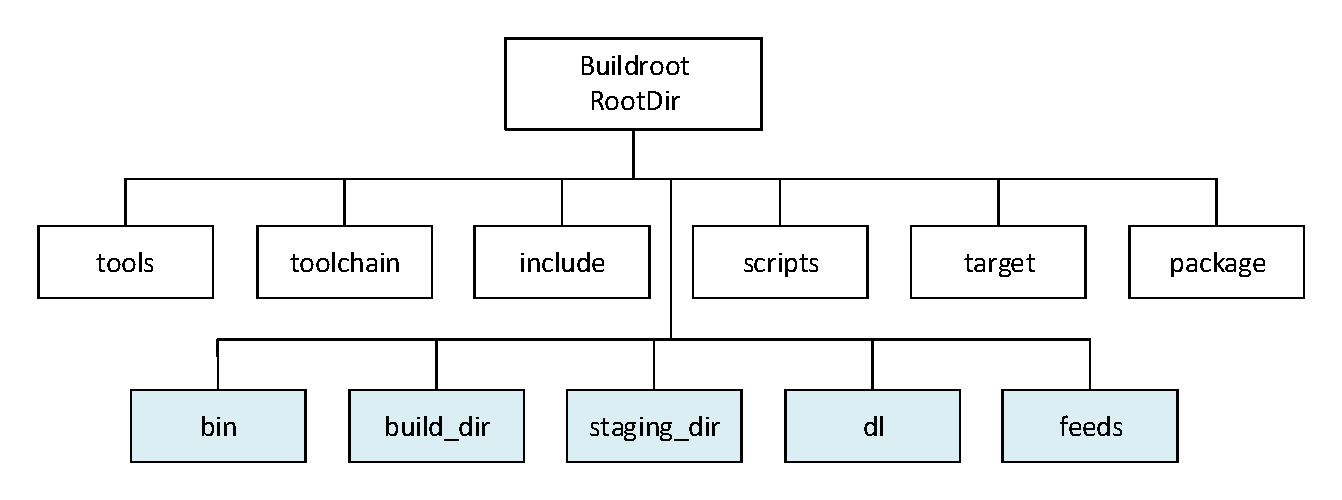
\includegraphics[width=1.0\textwidth]{openwrt-buildroot}
    \caption{
        \label{fig:openwrt-buildroot}
        Kiến trúc của OpenWrt Buildroot}
\end{figure}

Trong đó:
\begin{itemize}
\item \emph{tools} -- bao gồm tất cả các chỉ thị xây dựng để lấy về các công cụ xây dựng firmware.
\item \emph{toolchain} {-­‐} bao gồm các tất cả các chỉ thị xây dựng để lấy về tiêu đề nhân Linux, thư viện C, bin{-}utils, trình biên dịch và trình gỡ rối.
\item \emph{target} {-­‐} các chỉ thị xây dựng cho quá trình tạo bản chụp firmware và cho quá trình xây dựng nhân; biên dịch nhân và xây dựng bản chụp firmware.
\item \emph{package} -- OpenWrt Makefile và các bản vá cho tất cả các gói chính thức.
\item \emph{scripts} -- các script perl của hệ quản lý gói OpenWrt.
\item \emph{dl} -- thư mục chứa tất cả các gói tin cài đặt được tải về.
\item \emph{build\_dir} --  thư mục chứa các công cụ phục vụ người dùng được biên dịch chéo.
\item \emph{staging\_dir} -- thư mục chứa các công cụ biên dịch chéo.
\item \emph{feeds} -- thư mục chứa các cấu hình nguồn cài đặt.
\item \emph{bin} -- thư mục  chứa các bản chụp firmware sau biên dịch và tất cả các gói \emph{.ipk} được tạo ra.\\
\end{itemize}

Sau khi OpenWrt Buildroot được cấu hình thích hợp, nền tảng và kiến trúc đích được xác định, các gói phần mềm cho người dùng được lựa chọn, OpenWrt Buildroot sẽ thực hiện quá trình xây dựng firmware qua các bước chính như sau:

1. Tải về các công cụ biên dịch chéo, tiêu đề nhân, và các công cụ tương tự.

2. Thiết lập thư mục cho giai đoạn (\emph{staging\_dir/}). Đây là nơi mà các công cụ biên dịch chéo sẽ được cài đặt.   

3. Tạo thư mục tải về (mặc định là \emph{dl/}). Đây là nơi mà các gói cài đặt được tải về. 

4. Tạo thư mục xây dựng (\emph{build\_dir/}). Đây là nơi mà tất cả các công cụ phục vụ người dùng được biên dịch.

5. Tạo thư mục đích (mặc định là \emph{build\_dir/target-arch/root}) và bộ khung của tập tin hệ thống. Thư mục này sẽ chứa tập tin hệ thống cuối cùng. 

6. Cài đặt các gói phục vụ người dùng vào tập tin hệ thống gốc và nén toàn bộ tập tin hệ thống gốc với định dạng phù hợp. Bản chụp firmware cuối cùng được tạo trong \emph{bin/}.

\section{Kết chương}
Trong chương 2, đồ án đã trình bày về những kiến thức nền tảng và các kiến thức liên quan cho việc xây dựng đề tài. Qua đó, các phương pháp phát hiện xâm nhập nói chung và phát hiện xâm nhập trong mạng không dây nói riêng đã được làm rõ. Việc khảo sát các hệ thống đã được phát triển đã mang lại cái nhìn tổng quan về một số hệ thống phát hiện xâm nhập mạng không dây trên thế giới, cũng như thấy được ưu nhược điểm của chúng. Đồ án cũng nghiên cứu về Kismet Wireless và Snort, là những phần mềm phát hiện xâm nhập mã nguồn mở điển hình và đang được ứng dụng rộng rãi.

Từ những kết quả nghiên cứu nêu trên, đồ án sẽ thực hiện một ý tưởng đó là xây dựng một hệ thống phát hiện xâm nhập mạng không dây dựa trên sự kết hợp những tính năng nổi bật của Kismet Wireless và Snort, chi tiết thiết kế và hoạt động của hệ thống sẽ được trình bày ở chương tiếp theo.
